\documentclass{article}
\usepackage[utf8]{inputenc}
\usepackage[brazil]{babel}
\usepackage{graphicx}
\usepackage{amsmath, amssymb}
\usepackage{hyperref}
\usepackage{float}
\usepackage[a4paper, margin=1in]{geometry} 
\usepackage{setspace}
\onehalfspacing


\title{Fundamentos de Probabilidade e Estatística para Ciência de Dados}
\author{Exercícios Resolvidos das aulas do Prof. Dr. Francisco Rodrigues (ICMC-USP)}
\date{Agosto de 2025}

\begin{document}

% Capa personalizada
\begin{titlepage}
    \centering
    \vspace*{3cm}
    {\scshape\LARGE Universidade de São Paulo \par}
    \vspace{1cm}
    {\scshape\Large Instituto de Ciências Matemáticas e de Computação\par}
    \vspace{2.5cm}
    {\huge\bfseries Fundamentos de Probabilidade e Estatística para Ciência de Dados\par}
    \vspace{1cm}
    {\Large Resumo das aulas do Prof. Dr. Francisco Rodrigues\par}
    \vfill
    {\Large Bruna Zamith Santos\par}
    \vspace{0.5cm}
    {\large Agosto de 2025\par}
\end{titlepage}

% Sumário
\tableofcontents
\newpage

\section{Teoria dos Conjuntos}
\subsection{Exercício 1}
Sejam os conjuntos:
$$X = \{10, 20, 30\}, \quad Y = \{5, 10, 15, 20\}$$
Calcule:  
(a) $X \cup Y$
(b) $X \cap Y$  
(c) $X^c$

\vspace{0.5cm}
\textbf{Solução:}
\begin{itemize}
    \item[(a)] $X \cup Y = \{5, 10, 15, 20, 30\}$
    \item[(b)] $X \cap Y = \{10, 20\}$
    \item[(c)] $X^c$: depende do conjunto universo $U$.  
          Se considerarmos $U = \{5, 10, 15, 20, 30\}$, então  
          $$X^c = U \setminus X = \{5, 15\}.$$
\end{itemize}

\subsection{Exercício 2}
Sejam $A$ e $B$ dois eventos em um mesmo espaço amostral.  
Escreva na linguagem dos conjuntos:
(a) O evento $A$ ocorre, mas $B$ não ocorre.
(b) Nenhum dos dois eventos ocorre.  

\vspace{0.5cm}
\textbf{Solução:}
\begin{itemize}
    \item[(a)] Nesse caso, temos que selecionar a parte de $A$ que não está em $B$, pois apenas $A$ ocorre. Para resolvermos esse problema, podemos usar o diagrama de Venn, conforme mostrado na Figura~\ref{fig:ex_1_2}. Portanto, a área em cinza é dada por $$A \cap B^c,$$ isto é, $A$ ocorre e $B$ não ocorre.  
    \item[(b)] Temos que considerar a região que não está em $A$ e nem em $B$, isto é, $$A^c \cap B^c.$$ Essa região é a área externa aos dois círculos que representam os eventos, conforme observamos na Figura~\ref{fig:ex_1_2}.
\end{itemize}

\begin{figure}[H]
    \centering
    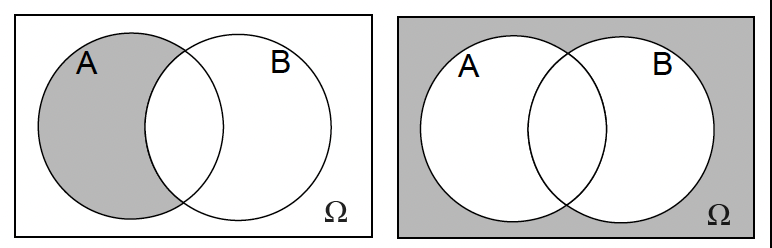
\includegraphics[width=0.6\textwidth]{figuras/ex_1_2.png}
    \caption{Exercício 1.2.}
    \label{fig:ex_1_2}
\end{figure}

\section{Conceitos de Probabilidade}
\subsection{Exercício 1}
Imagine uma urna com 5 bolas brancas e 3 pretas. Qual
é a probabilidade de retirar uma bola branca?

\vspace{0.5cm}
\textbf{Solução:}

Seja o evento $A$: ``retirar uma bola branca''.  
Temos 5 bolas brancas e 3 bolas pretas, logo o total é $5+3=8$.  
Portanto,
    $$
    P(A) = \frac{5}{5+3} = \frac{5}{8}.
    $$

\subsection{Exercício 2}
Uma urna contém fichas numeradas de 1 a 20. Supondo que alguém escolha uma dessas fichas ao acaso, qual a probabilidade de que a ficha escolhida contenha um número maior que 9?

\vspace{0.5cm}
\textbf{Solução:}

As fichas estão enumeradas de 1 a 20, então há 20 fichas no total. Os números maiores que 9 são 10, 11, 12, 13, 14, 15, 16, 17, 18, 19 e 20. Portanto, há 11 fichas que atendem a essa condição.  
Vamos definir o evento $A$ como ``escolher uma ficha com um número maior que 9''.  
Logo,
    $$
    P(A) = \frac{|A|}{|\Omega|} = \frac{11}{20} = 0.55.
    $$
Portanto, a probabilidade de escolher uma ficha que contenha um número maior que 9 é $11/20$, ou 55\%.

\subsection{Exercício 3}
Considere o problema proposto pelo matemático suíço Jakob Bernoulli (1654-1705). Uma urna contém 3.000 bolas brancas e 2.000 bolas pretas. Calcule a probabilidade de retirar uma bola preta da urna.

\vspace{0.5cm}
\textbf{Solução:}

A probabilidade de sortearmos uma bola preta, usando a definição clássica, é dada por:
    $$
    P(A) = \frac{|A|}{|\Omega|} = \frac{n(A)}{n(\Omega)} = 
    \frac{2000}{2000 + 3000} = 0.4,
    $$
onde $A$ é o evento ``retirar uma bola preta''.  
Se simulamos esse experimento, considerando o código a seguir, realizando a retirada 100 vezes, obtemos o valor $f_A = 0,38$, sendo $f_A$ a frequência que o evento $A$ ocorre.  
Notem que esse valor varia de uma execução para outra, pois estamos considerando um experimento aleatório.

\subsection{Exercício 4}
Em uma escola particular, dentre todos os alunos que
procuram ajuda, 63\% precisam de aulas de reforço em matemática, 34\% precisam de ajuda em inglês e 27\% precisam de aulas adicionais tanto em matemáica quanto em inglês. Qual é a percentagem de alunos que precisam de ajuda em matemática ou em inglês (ou em ambas disciplinas)?

\vspace{0.5cm}
\textbf{Solução:}

Sejam os eventos:
\begin{itemize}
    \item $A$: ``precisam de ajuda em matemática'';
    \item $B$: ``precisam de ajuda em inglês''
\end{itemize}

Pela fórmula da probabilidade da união de dois eventos:
    $$
    P(A \cup B) = P(A) + P(B) - P(A \cap B)
    $$

Substituindo os valores:
    $$
    P(A \cup B) = 0.63 + 0.34 - 0.27 = 0.70
    $$

\section{Teorema de Bayes}
\subsection{Exercício 1}
Calcule $P(A|B)$ onde:

\begin{itemize}
    \item $\Omega = \{1,2,3,\ldots,15\}$,
    \item $A$: ``sai um valor maior do que 5'',
    \item $B$: ``sai um valor par'',
    \item $A \subset \Omega$ e $B \subset \Omega$.
\end{itemize}

\vspace{0.5cm}
\textbf{Solução:}
Observando os conjuntos, temos que $A$ tem 10 elementos, enquanto $B$ possui 7:
    $$
    P(A) = \frac{10}{15} = \frac{2}{3}, 
    \quad
    P(B) = \frac{7}{15}.
    $$

Além disso:
    $$
    A \cap B = \{6,8,10,12,14\}.
    $$

Assim,
    $$
    P(A|B) = \frac{P(A \cap B)}{P(B)} 
    = \frac{\tfrac{5}{15}}{\tfrac{7}{15}} 
    = \frac{5}{7}.
    $$

Logo, a ocorrência de $B$ aumenta a probabilidade de observação de $A$, isto é, $P(A|B) > P(A)$.

\subsection{Exercício 2}
Uma empresa possui 100 funcionários. Alguns desses funcionários possuem curso superior (evento $A$), enquanto que outros, apenas o fundamental (evento $B$). Alguns são estagiários (evento $C$), enquanto que outros são efetivos (evento $D$). A tabela a seguir mostra a distribuição dos funcionários de acordo com essas categorias:

\vspace{0.5cm}
\begin{center}
\begin{tabular}{lccc}
\hline
 & A & B & Total \\
\hline
C & 40 & 30 & 70 \\
D & 20 & 10 & 30 \\
\hline
Total & 60 & 40 & 100 \\
\hline
\end{tabular}
\end{center}

Um funcionário é selecionado aleatoriamente e verifica-se que é estagiário. Qual é a probabilidade do funcionário ter curso superior?

\vspace{0.5cm}
\textbf{Solução:}
Queremos calcular $P(A|C)$:
    $$
    P(A|C) = \frac{P(A \cap C)}{P(C)}.
    $$
    
Da tabela:  
\begin{itemize} 
    \item $P(A \cap C) = \tfrac{40}{100}$  
    \item $P(C) = \tfrac{70}{100}$  
\end{itemize}

Logo,
    $$
    P(A|C) = \frac{\tfrac{40}{100}}{\tfrac{70}{100}} = \frac{40}{70} = \frac{4}{7} \approx 0.571.
    $$
Portanto, a probabilidade de que o funcionário tenha curso superior dado que é estagiário é de aproximadamente 57\%.

\subsection{Exercício 3}
Suponha que dois dados sejam lançados. Sejam os eventos:
\begin{itemize}
    \item $A$: ``a soma dos dados é igual a 6''.  
    \item $B$: ``o primeiro dado resultou no valor 4''.  
\end{itemize}

Esses eventos são independentes?

\vspace{0.5cm}
\textbf{Solução:}
Temos:
    $$
    P(A \cap B) = P((4,2)) = \frac{1}{36} \approx 0.028.
    $$

Enquanto isso:
    $$
    P(A) = \frac{5}{36}, \quad P(B) = \frac{6}{36}, 
    $$

portanto:
    $$
    P(A) \cdot P(B) = \frac{5}{36} \cdot \frac{6}{36} = \frac{30}{1296} \approx 0.023.
    $$

Como $P(A \cap B) \neq P(A)P(B)$, concluímos que $A$ e $B$ não são independentes.

\subsection{Exercício 4}
Moedas de ouro e prata são colocadas em 3 urnas, conforme a tabela a seguir:
\vspace{0.5cm}
    \begin{center}
    \begin{tabular}{lcc}
    \hline
    Urna & Moedas de ouro & Moedas de prata \\
    \hline
    I    & 4 & 8 \\
    II   & 3 & 9 \\
    III  & 6 & 6 \\
    \hline
    \end{tabular}
    \end{center}

Cada urna tem uma probabilidade de ser escolhida:
    $$
    P(I) = \tfrac{1}{2}, \quad P(II) = \tfrac{1}{4}, \quad P(III) = \tfrac{1}{4}.
    $$

Qual é a probabilidade de selecionarmos uma moeda de ouro?

\vspace{0.5cm}
\textbf{Solução:}
Definimos o evento $A$: ``escolher uma moeda de ouro''.  
Usando probabilidade total:
    $$
    P(A) = P(A|I)P(I) + P(A|II)P(II) + P(A|III)P(III).
    $$

Calculando cada termo:  
\begin{itemize}
    \item $P(A|I) = \tfrac{4}{12}$  
    \item $P(A|II) = \tfrac{3}{12}$  
    \item $P(A|III) = \tfrac{6}{12}$  
\end{itemize}

Substituindo:
    $$
    P(A) = \frac{4}{12}\cdot \frac{1}{2} + \frac{3}{12}\cdot \frac{1}{4} + \frac{6}{12}\cdot \frac{1}{4}.
    $$
    
    $$
    P(A) = \frac{1}{6} + \frac{1}{16} + \frac{1}{8} = \frac{17}{48} \approx 0.35
    $$

Portanto, a probabilidade é de aproximadamente 35\%.

\subsection{Exercício 5}
Um laboratório que faz testes sanguíneos apresenta eficácia de 95\% na detecção de uma certa doença quando, de fato, a pessoa está doente (verdadeiro positivo).  
A taxa de falsos positivos, ou seja, quando o teste afirma que o paciente tem a doença, embora seja saudável, é de 2\%.  
Se 0,1\% da população realmente tem a doença, qual é a probabilidade de que uma pessoa tenha a doença dado que o teste foi positivo?

\vspace{0.5cm}
\textbf{Solução:}
Vamos definir os eventos:  
\begin{itemize}
    \item $A$: ``o paciente tem a doença''  
    \item $B$: ``o teste foi positivo''  
\end{itemize}

Usando as informações do problema:
    $$
    P(B|A) = 0.95, 
    \quad P(A) = 0.001,
    \quad P(B|A^c) = 0.02
    $$

Usando o Teorema de Bayes:
    $$
    P(A|B) = \frac{P(B|A)P(A)}{P(B|A)P(A) + P(B|A^c)P(A^c)}.
    $$

Substituindo:
    $$
    P(A|B) = \frac{0.95 \times 0.001}{0.95 \times 0.001 + 0.02 \times 0.999}
    = 0.045
    $$

Portanto, a probabilidade de que o paciente realmente esteja doente dado que o teste foi positivo é de 4,5\%.  
Mesmo sendo baixa, essa probabilidade é 45 vezes maior que a prevalência inicial (0,1\%), mostrando o impacto do teste.

\subsection{Exercício 6}
Suponha que temos três moedas idênticas no formato, mas sendo que a primeira moeda tem duas caras, a segunda tem duas coroas e a terceira é uma moeda justa, com uma cara em uma face e uma coroa na outra. As moedas são misturadas em uma caixa. Se retiramos uma moeda e mostramos uma cara, qual é a probabilidade de que a outra face contenha uma coroa, ou seja, qual a probabilidade de que essa seja a moeda justa?

\vspace{0.5cm}
\textbf{Solução:} Vamos definir os eventos:
\begin{itemize}
    \item $CC$: ``a moeda tem duas caras'',
    \item $RR$: ``a moeda tem duas coroas'',
    \item $CR$: ``a moeda é justa'',
    \item $C$: ``é mostrada uma cara''.
\end{itemize}

Usando o teorema de Bayes, a probabilidade de que a moeda é justa dado que uma cara foi mostrada é calculada por:
    $$
    P(CR|C) = \frac{P(C|CR)P(CR)}{P(C|CR)P(CR) + P(C|CC)P(CC) + P(C|RR)P(RR)}.
    $$
    
As probabilidades são dadas por:
    $$
    P(C|CR) = \tfrac{1}{2}, \quad P(C|CC) = 1, \quad P(C|RR) = 0.
    $$
    
Substituindo os valores:
    $$
    P(CR|C) = \frac{\tfrac{1}{2}\times \tfrac{1}{3}}{\tfrac{1}{2}\times \tfrac{1}{3} + 1\times \tfrac{1}{3} + 0\times \tfrac{1}{3}} = \tfrac{1}{3}.
    $$

\subsection{Exercício 7}
Suponha que cinco lâmpadas perfeitas são misturadas com duas lâmpadas defeituosas, que não funcionam. Para encontrar as lâmpadas defeituosas, temos que testar uma a uma, sem substituição. Qual é a probabilidade de encontrarmos as duas lâmpadas defeituosas nos dois primeiros testes?

\vspace{0.5cm}
\textbf{Solução:} Seja o evento $D_i$: ``selecionamos a lâmpada defeituosa no teste $i$''. Assim, queremos calcular:
    $$
    P(D_1 \cap D_2),
    $$
isto é, a probabilidade de que as duas primeiras lâmpadas sejam defeituosas.

Pela regra da probabilidade condicional:
    $$
    P(D_1 \cap D_2) = P(D_1) P(D_2|D_1).
    $$

Como temos 7 lâmpadas (2 defeituosas), temos:
    $$
    P(D_1) = \frac{2}{7}, \quad P(D_2|D_1) = \frac{1}{6}.
    $$
    
Logo:
    $$
    P(D_1 \cap D_2) = \frac{2}{7} \cdot \frac{1}{6} = \frac{1}{21}.
    $$

\subsection{Exercício 8}
Temos duas urnas, I e II. A urna I contém 2 bolas pretas e 3 bolas brancas. A urna II contém 1 bola preta e 1 bola branca. Uma urna é selecionada ao acaso e uma de suas bolas é escolhida. Dado que uma bola preta foi retirada, qual é a probabilidade de que a urna I foi escolhida?

\vspace{0.5cm}
\textbf{Solução:} Definimos os eventos:
\begin{itemize}
    \item $I$: ``a urna I foi escolhida'',
    \item $A$: ``uma bola preta foi retirada''.
\end{itemize}

Pelo teorema de Bayes:
    $$
    P(I|A) = \frac{P(A|I)P(I)}{P(A)}.
    $$

Mas:
    $$
    P(A) = P(A \cap I) + P(A \cap I^c) = P(A|I)P(I) + P(A|I^c)P(I^c).
    $$

Temos:
    $$
    P(A|I) = \tfrac{2}{5}, \quad P(A|I^c) = \tfrac{1}{2}, \quad P(I)=P(I^c)=\tfrac{1}{2}.
    $$

Logo:
    $$
    P(A) = \tfrac{2}{5}\cdot\tfrac{1}{2} + \tfrac{1}{2}\cdot\tfrac{1}{2} 
    = \tfrac{1}{5} + \tfrac{1}{4} 
    = \tfrac{9}{20}.
    $$

Portanto:
    $$
    P(I|A) = \frac{P(A|I)P(I)}{P(A)} 
    = \frac{\tfrac{2}{5}\cdot\tfrac{1}{2}}{\tfrac{9}{20}} 
    = \frac{1/5}{9/20} 
    = \tfrac{4}{9}.
    $$

\section{Variáveis Aleatórias}
\subsection{Exercício 1}
Suponha que lançamos três moedas. Se definirmos o evento $C$ para representar uma cara observada e $R$ para uma coroa, teremos os seguintes resultados possíveis:
    $$
    \Omega = \{(C,C,C), (C,C,R), (C,R,C), (R,C,C), (R,R,C), (R,C,R), (C,R,R), (R,R,R)\}.
    $$
A partir do espaço amostral e dos eventos, calcule diversas quantidades como o número de caras, o número de saídas em que as faces são diferentes, ou o lucro médio se cada cara resulta em um ganho de 10 reais.  

\vspace{0.5cm}
\textbf{Solução:}
Se definirmos uma função que retorna o número de caras e assumirmos que cada cara sai com probabilidade $p$, podemos calcular essas quantidades usando a tabela.
    $$
    \begin{array}{|c|c|c|}
    \hline
    \text{Saída} & \text{Número de caras} & \text{Probabilidade} \\
    \hline
    (C,C,C) & 3 & p^3 \\
    (C,C,R) & 2 & p^2(1-p) \\
    (C,R,C) & 2 & p^2(1-p) \\
    (R,C,C) & 2 & p^2(1-p) \\
    (R,C,R) & 1 & p(1-p)^2 \\
    (R,R,C) & 1 & p(1-p)^2 \\
    (C,R,R) & 1 & p(1-p)^2 \\
    (R,R,R) & 0 & (1-p)^3 \\
    \hline
    \end{array}
    $$

\subsection{Exercício 2}
Duas bolas são retiradas sucessivamente, sem reposição, de uma caixa que contém 10 bolas vermelhas e 5 azuis.  
Seja a variável aleatória:
    $$
    X : \text{``número de bolas vermelhas retiradas no experimento''}.
    $$

Determine a distribuição de probabilidade de $X$.

\vspace{0.5cm}
\textbf{Solução:} 
Sejam os eventos:
    $$
    \begin{cases}
    V_i: \text{``uma bola vermelha retirada na tentativa $i$''} \\
    A_i: \text{``uma bola azul retirada na tentativa $i$''}
    \end{cases}
    $$

A probabilidade associada a cada saída possível do experimento é calculada a seguir. Por exemplo, para duas bolas azuis retiradas:
    $$
    P(X = 0) = P((A_1, A_2)) = \frac{5}{15} \times \frac{4}{14} = \frac{20}{210} = \frac{2}{21}.
    $$

Portanto, temos a seguinte tabela:
    $$
    \begin{array}{|c|c|c|}
    \hline
    \text{Saída} & X = x & P(X = x) \\
    \hline
    (V_1, A_2) & 1 & \tfrac{10}{15} \times \tfrac{5}{14} = \tfrac{5}{21} \\
    (A_1, V_2) & 1 & \tfrac{5}{15} \times \tfrac{10}{14} = \tfrac{5}{21} \\
    (V_1, V_2) & 2 & \tfrac{10}{15} \times \tfrac{9}{14} = \tfrac{9}{21} \\
    (A_1, A_2) & 0 & \tfrac{5}{15} \times \tfrac{4}{14} = \tfrac{2}{21} \\
    \hline
    \end{array}
    $$

Com isso, construímos a distribuição de probabilidade de $X$, que é dada por:
    $$
    \begin{array}{|c|c|c|c|}
    \hline
    X & 0 & 1 & 2 \\
    \hline
    P(X = x_i) & \tfrac{2}{21} & \tfrac{10}{21} & \tfrac{9}{21} \\
    \hline
    \end{array}
    $$

Notem que:
    $$
    \sum_{k=0}^{2} P(X = k) = 1.
    $$

\subsection{Exercício 3}
Em um cassino da cidade, um novo jogo de dados é apresentado. Nesse jogo, um jogador paga 10 reais para participar. O jogador e a banca lançam cada um o seu dado e a seguinte regra de premiação é estabelecida:
\begin{itemize}
    \item Se o ponto do jogador é maior, ele ganha 3 vezes a diferença entre o seu ponto e o obtido pelo oponente.
    \item Se o ponto do jogador é menor ou igual ao do oponente, ele não ganha nada.
\end{itemize}
Esse jogo é favorável ao jogador?

\vspace{0.5cm}
\textbf{Solução:}
Vamos definir as variáveis aleatórias:
\begin{itemize}
    \item $G$: ``ganho bruto do jogador'' 
    \item $X$: ``valor obtido pelo oponente''
    \item $Y$: ``valor obtido pelo jogador''
\end{itemize}

Considerando a regra de premiação, podemos escrever a variável aleatória $G$ em função de $X$ e $Y$:
    $$
    G =
    \begin{cases}
    3(Y - X), & \text{se } Y > X \\
    0, & \text{se } Y \leq X
    \end{cases}
    $$
A distribuição de probabilidade de $G$ é dada por:
    $$
    \begin{array}{|c|c|c|c|c|c|c|}
    \hline
    G & 0 & 3 & 6 & 9 & 12 & 15 \\
    \hline
    P(G = g_i) & \tfrac{21}{36} & \tfrac{5}{36} & \tfrac{4}{36} & \tfrac{3}{36} & \tfrac{2}{36} & \tfrac{1}{36} \\
    \hline
    \end{array}
    $$
    
Portanto, para ter lucro é preciso que $P(G \geq 10)$, pois o jogador apostou 10 reais:
    $$
    P(G \geq 10) = P(G = 12) + P(G = 15) 
    = \tfrac{2}{36} + \tfrac{1}{36} 
    = \tfrac{3}{36} 
    = \tfrac{1}{12} 
    = 0.08
    $$

Assim, a chance de lucro é muito pequena. Logo, não vale a pena jogar esse jogo.

\subsection{Exercício 4}
Seja $X$ uma variável aleatória contínua com função de densidade de probabilidade:
    $$
    f(x) =
    \begin{cases}
    2x, & 0 < x < 1, \\
    0, & \text{caso contrário}.
    \end{cases}
    $$

Verifique se $f(x)$ é uma função de densidade de probabilidade e calcule a probabilidade $P(X \geq 1/2)$.

\vspace{0.5cm}
\textbf{Solução:} Para que $f(x)$ seja uma função de densidade de probabilidade, temos que:
    $$
    f(x) \geq 0, \quad \forall x \in \mathbb{R}.
    $$
Além disso,
    $$
    \int_{-\infty}^{\infty} f(x)\, dx 
    = \int_{-\infty}^{0} f(x)\, dx + \int_{0}^{1} f(x)\, dx + \int_{1}^{\infty} f(x)\, dx
    = \int_{0}^{1} 2x \, dx.
    $$
    $$
    \int_{0}^{1} 2x \, dx = \left. \frac{2x^2}{2} \right|_{0}^{1} = 1^2 - 0^2 = 1.
    $$

Portanto, $f(x)$ é uma f.d.p. válida.

Agora vamos calcular $P(X \geq 1/2)$:
    $$
    P(X \geq 1/2) = \int_{1/2}^{\infty} f(x) \, dx = \int_{1/2}^{1} 2x \, dx
    = \left. \frac{2x^2}{2} \right|_{1/2}^{1}
    = 1 - \frac{1}{4} = \frac{3}{4}.
    $$

\subsection{Exercício 5}
Seja $X$ uma variável aleatória contínua com função de densidade de probabilidade:
    $$
    f(x) = 
    \begin{cases}
    C(4x - 2x^2), & 0 \leq x \leq 2, \\
    0, & \text{caso contrário}.
    \end{cases}
    $$

Determine o valor da constante $C$ e calcule $P(X > 1)$.

\vspace{0.5cm}
\textbf{Solução:} Como $f(x)$ é uma função de densidade de probabilidade, temos:
    $$
    \int_{-\infty}^{\infty} f(x) \, dx = 1 \;\;\;\; \Longrightarrow \;\;\;\; \int_{0}^{2} C(4x - 2x^2)\, dx = 1
    $$
    $$
    C \left[ \frac{4x^2}{2} - \frac{2x^3}{3} \right]_{x=0}^{2} = 1 \;\;\;\; \Longrightarrow \;\;\;\; C = \frac{3}{8}.
    $$

Podemos calcular $P(X > 1)$:
    $$
    P(X > 1) = \int_{1}^{2} \frac{3}{8}(4x - 2x^2)\, dx 
    = \frac{3}{8} \left( \frac{4x^2}{2} - \frac{2x^3}{3} \right)\Big|_{1}^{2}
    = \frac{1}{2}.
    $$

\subsection{Exercício 6}
Seja $X$ uma variável aleatória contínua com função de densidade de probabilidade:
    $$
    f(x) = 
    \begin{cases} 
    2x, & 0 < x < 1, \\[6pt]
    0, & \text{caso contrário}.
    \end{cases}
    $$

Calcule $P(X > 1/2 \mid X > 1/4)$.

\vspace{0.5cm}
\textbf{Solução:} Usando a definição de probabilidade condicional, temos:
    $$
    P(X > 1/2 \mid X > 1/4) = \frac{P(X > 1/2, X > 1/4)}{P(X > 1/4)}.
    $$
O termo $P(X > 1/2, X > 1/4)$ indica a probabilidade de que $X > 1/2$ e $X > 1/4$, ou seja, é a probabilidade da interseção desses dois intervalos:
    $$
    \{X > 1/2 \cap X > 1/4\} \equiv \{X > 1/2\}.
    $$

Assim,
    $$
    P(X > 1/2 \mid X > 1/4) = \frac{P(X > 1/2)}{P(X > 1/4)}.
    $$  
    $$
    P(X > 1/2 \mid X > 1/4) = \frac{\int_{1/2}^{1} 2x \, dx}{\int_{1/4}^{1} 2x \, dx}.
    $$

Calculando as integrais:
    $$
    \int_{1/2}^{1} 2x \, dx = \left[ x^2 \right]_{1/2}^{1} = 1 - \frac{1}{4} = \frac{3}{4}.
    $$
    $$
    \int_{1/4}^{1} 2x \, dx = \left[ x^2 \right]_{1/4}^{1} = 1 - \frac{1}{16} = \frac{15}{16}.
    $$

Portanto:
    $$
    P(X > 1/2 \mid X > 1/4) = \frac{\tfrac{3}{4}}{\tfrac{15}{16}} = \frac{4}{5} = 0.8
    $$

\section{Função de Distribuição}
\subsection{Exercício 1}
Duas bolas são retiradas sucessivamente, sem reposição, de uma caixa que contém 5 bolas vermelhas e 4 pretas.  
Seja $X$ a variável aleatória ``número de bolas vermelhas retiradas no experimento''.  
Determine a distribuição de probabilidade da variável aleatória $X$ e sua função de distribuição.

\vspace{0.5cm}
\textbf{Solução:} Sejam os eventos:
    $$
    \begin{cases}
    P_i : \text{``bola preta na retirada $i$''}, \\
    V_i : \text{``bola vermelha na retirada $i$''}.
    \end{cases}
    $$
    
A probabilidade associada a cada saída possível é calculada da seguinte forma:
    $$
    P(X = 0) = P((P_1, P_2)) = \frac{4}{9} \cdot \frac{3}{8} = \frac{12}{72}.
    $$  
    $$
    P(X = 1) = P((V_1, P_2) \cup (P_1, V_2)) 
    = \frac{5}{9}\cdot \frac{4}{8} + \frac{4}{9}\cdot \frac{5}{8} 
    = \frac{40}{72}.
    $$
    $$
    P(X = 2) = P((V_1, V_2)) = \frac{5}{9} \cdot \frac{4}{8} = \frac{20}{72}.
    $$
    
Assim, a distribuição de probabilidade de $X$ é dada por:
    $$
    \begin{array}{|c|c|c|c|}
    \hline
    X & 0 & 1 & 2 \\
    \hline
    P(X=x) & \tfrac{12}{72} & \tfrac{40}{72} & \tfrac{20}{72} \\
    \hline
    \end{array}
    $$

\vspace{0.5cm}
Para calcular a função de distribuição acumulada $F(x) = P(X \leq x)$, somamos as probabilidades em cada intervalo:
    $$
    F(x) =
    \begin{cases}
    0, & x < 0, \\[6pt]
    \frac{12}{72}, & 0 \leq x < 1, \\[6pt]
    \frac{52}{72}, & 1 \leq x < 2, \\[6pt]
    1, & x \geq 2.
    \end{cases}
    $$

\subsection{Exercício 2}
Seja $X$ uma variável aleatória contínua com função de densidade de probabilidade:
    $$
    f(x) =
    \begin{cases}
    \frac{1}{b-a}, & a \leq x \leq b, \\
    0, & \text{caso contrário}.
    \end{cases}
    $$

Determine a função de distribuição de $X$.

\vspace{0.5cm}
\textbf{Solução:} Usando a definição da função de distribuição acumulada:
\begin{itemize}
    \item Se $x < a$:
    $$
    F(x) = \int_{-\infty}^{a} f(s) \, ds = 0.
    $$
    \item Se $a \leq x < b$:
    $$
    F(x) = P(X \leq x) = \int_{-\infty}^{x} f(s) \, ds = \int_{a}^{x} \frac{1}{b-a} \, ds 
    = \frac{x-a}{b-a}.
    $$
    \item Se $x \geq b$:
    $$
    F(x) = \int_{-\infty}^{x} f(s) \, ds = \int_{a}^{b} \frac{1}{b-a} \, ds = 1.
    $$
\end{itemize}

Portanto:
    $$
    F(x) =
    \begin{cases}
    0, & x < a, \\
    \frac{x-a}{b-a}, & a \leq x < b, \\
    1, & x \geq b.
    \end{cases}
    $$

\subsection{Exercício 3}
Seja 
    $$
    F(x) = 1 - e^{-\lambda x}, \quad x \geq 0,
    $$
e $F(x) = 0$ para $x < 0$. Calcule $f(x)$.
    
\vspace{0.5cm}
\textbf{Solução:} Para encontrar $f(x)$ derivamos $F(x)$ em relação a $x$:
    $$
    f(x) = \frac{d}{dx} F(x).
    $$
    
Derivando:
    $$
    f(x) = \frac{d}{dx} \left( 1 - e^{-\lambda x} \right),
    $$
    $$
    f(x) = 0 - (-\lambda e^{-\lambda x}),
    $$
    $$
    f(x) = \lambda e^{-\lambda x}, \quad x \geq 0.
    $$
    
Para $x < 0$, como $F(x) = 0$, temos $f(x) = 0$.

Portanto:
    $$
    f(x) =
    \begin{cases}
    \lambda e^{-\lambda x}, & x \geq 0, \\
    0, & x < 0.
    \end{cases}
    $$

\section{Esperança}
\subsection{Exercício 1}
Seja $X$ o valor que sai na face superior de um dado.  
Calcule o valor esperado de $X$.  

\vspace{0.5cm}
\textbf{Solução:}
A distribuição de probabilidade de $X$ é dada por:
    $$
    \begin{array}{|c|c|c|c|c|c|c|}
    \hline
    X & 1 & 2 & 3 & 4 & 5 & 6 \\
    \hline
    P(X = x_i) & \tfrac{1}{6} & \tfrac{1}{6} & \tfrac{1}{6} & \tfrac{1}{6} & \tfrac{1}{6} & \tfrac{1}{6} \\
    \hline
    \end{array}
    $$
    $$
    E(X) = 1 \cdot \tfrac{1}{6} + 2 \cdot \tfrac{1}{6} + 3 \cdot \tfrac{1}{6} + 4 \cdot \tfrac{1}{6} + 5 \cdot \tfrac{1}{6} + 6 \cdot \tfrac{1}{6} = \tfrac{7}{2} = 3.5
    $$

Note que $3,5$ não é um valor possível de $X$.

\subsection{Exercício 2}
Uma padaria produz pães que proporcionam um lucro de R\$1.00, quando vendidos, ou um prejuízo de R\$0.50, caso não sejam vendidos.  
Se a probabilidade de vender um pão é igual a $0.8$, qual o lucro médio da padaria?

\vspace{0.5cm}
\textbf{Solução:}
A distribuição de probabilidade do lucro é dada na tabela:
    $$
    \begin{array}{|c|c|c|}
    \hline
    X & -0,5 & 1,0 \\
    \hline
    P(X = x_i) & 0,2 & 0,8 \\
    \hline
    \end{array}
    $$

Assim, o lucro médio é:
    $$
    E[X] = 1 \cdot 0.8 - 0.5 \cdot 0.2 = 0.7
    $$

Portanto, o lucro esperado por cada pão vendido é igual a R\$0.70.

\subsection{Exercício 3}
A variável aleatória $X$ tem função de densidade de probabilidade dada por:
    $$
    f(x) =
    \begin{cases}
    \dfrac{x^2}{3}, & -1 < x < 2, \\[6pt]
    0, & \text{caso contrário}.
    \end{cases}
    $$

Calcule o valor esperado de $X$.

\vspace{0.5cm}
\textbf{Solução:}
    $$
    E[X] = \int_{-\infty}^{\infty} x f(x) dx 
    = \int_{-1}^{2} x \cdot \frac{x^2}{3}\, dx
    = \int_{-1}^{2} \frac{x^3}{3}\, dx
    = \left. \frac{x^4}{12} \right|_{-1}^{2}
    = \frac{15}{12} = 1.25
    $$

\subsection{Exercício 4}
Lançamos dois dados e observamos a variável aleatória $X$, que é igual a $1$ se a soma dos valores for par, ou igual a $0$, caso contrário.  
Calcule a esperança de $g(X) = X + 2$.

\vspace{0.5cm}
\textbf{Solução:}
Há $36$ saídas possíveis. Assim:
    $$
    \begin{array}{|c|c|c|}
    \hline
    X & 0 & 1 \\
    \hline
    P(X = x_i) & \tfrac{18}{36} & \tfrac{18}{36} \\
    \hline
    \end{array}
    $$

O valor esperado é:
    $$
    E[g(X)] = E[X+2] = \sum_{k=0}^{1} (k+2) P(X=k).
    $$
    $$
    E[g(X)] = (0+2)\cdot \tfrac{18}{36} + (1+2)\cdot \tfrac{18}{36}
    = \frac{36}{36} + \frac{54}{36} = \frac{90}{36} = 2.5
    $$

\subsection{Exercício 5}
A variável aleatória $X$ tem função de densidade de probabilidade dada por:
    $$
    f(x) = 
    \begin{cases}
    \dfrac{x^2}{3}, & -1 < x < 2, \\
    0, & \text{caso contrário}.
    \end{cases}
    $$
Calcule o valor esperado de $g(X) = 2X + 1$.

\vspace{0.5cm}
\textbf{Solução:}
    $$
    E[g(X)] = \int_{-1}^2 (2x+1)\dfrac{x^2}{3}\, dx 
    = \dfrac{2x^4}{12} + \dfrac{x^3}{9}\Bigg|_{-1}^2
    = 3.5
    $$

\subsection{Exercício 6}
Se uma variável aleatória $X$ apresenta valor esperado $E[X] = 2$, calcule $E[2X+5]$.

\vspace{0.5cm}
\textbf{Solução:}
    $$
    E[2X+5] = 2E[X] + 5 = 2 \times 2 + 5 = 9.
    $$

\section{Momento}
\subsection{Exercício 1}
Sejam as variáveis aleatórias $X$ e $Y$ com distribuições de probabilidade:
    $$
    \begin{array}{c|ccccc}
    X & -2 & -1 & 0 & 1 & 2 \\ \hline
    P(X=x) & \tfrac{1}{5} & \tfrac{1}{5} & \tfrac{1}{5} & \tfrac{1}{5} & \tfrac{1}{5}
    \end{array}
    $$
    
    $$
    \begin{array}{c|ccccc}
    Y & -2 & -1 & 0 & 1 & 2 \\ \hline
    P(Y=y) & 0 & \tfrac{1}{4} & \tfrac{1}{2} & \tfrac{1}{4} & 0
    \end{array}
    $$

Calcule $E[X], \; E[Y], \; E[X^2] \; \text{e} \; E[Y^2]$.

\vspace{0.5cm}
\textbf{Solução:} Os valores esperados de $X$ e $Y$:
    $$
    E[X] = -2 \cdot \tfrac{1}{5} - 1 \cdot \tfrac{1}{5} + 0 \cdot \tfrac{1}{5} + 1 \cdot \tfrac{1}{5} + 2 \cdot \tfrac{1}{5} = 0,
    $$
    $$
    E[Y] = -2 \cdot 0 - 1 \cdot \tfrac{1}{4} + 0 \cdot \tfrac{1}{2} + 1 \cdot \tfrac{1}{4} + 2 \cdot 0 = 0.
    $$

Portanto, $X$ e $Y$ apresentam o mesmo valor esperado.  
Vamos calcular o segundo momento de $X$ e $Y$:
    $$
    E[X^2] = (-2)^2 \cdot \tfrac{1}{5} + (-1)^2 \cdot \tfrac{1}{5} + 0^2 \cdot \tfrac{1}{5} + 1^2 \cdot \tfrac{1}{5} + 2^2 \cdot \tfrac{1}{5} = \tfrac{10}{5} = 2,
    $$
    $$
    E[Y^2] = (-2)^2 \cdot 0 + (-1)^2 \cdot \tfrac{1}{4} + 0^2 \cdot \tfrac{1}{2} + 1^2 \cdot \tfrac{1}{4} + 2^2 \cdot 0 = \tfrac{2}{4} = 0.5
    $$

\section{Variância}
\subsection{Exercício 1}
Seja a v.a. $X$ cuja distribuição de probabilidade é dada a seguir. Calcule $V(X)$.
    $$
    \begin{array}{c|cccc}
    X & 0 & 1 & 2 & 3 \\ \hline
    P(X = x_i) & 0.51 & 0.38 & 0.10 & 0.01
    \end{array}
    $$

\vspace{0.5cm}
\textbf{Solução:}
Temos:
    $$
    E[X] = 0 \times 0.51 + 1 \times 0.38 + 2 \times 0.10 + 3 \times 0.01 = 0.61,
    $$
    $$
    E[X^2] = 0^2 \times 0.51 + 1^2 \times 0.38 + 2^2 \times 0.10 + 3^2 \times 0.01 = 0.87
    $$

Logo,
    $$
    V(X) = E[X^2] - (E[X])^2 = 0.87 - (0.61)^2 = 0.498
    $$

\subsection{Exercício 2}
Seja $X$ uma variável aleatória contínua com função de distribuição de probabilidade:
    $$
    f(x) =
    \begin{cases}
    x, & 0 \leq x \leq 1, \\
    2 - x, & 1 < x \leq 2, \\
    0, & \text{caso contrário}.
    \end{cases}
    $$

Calcule a variância de $X$.

\vspace{0.5cm}
\textbf{Solução:}

Vamos calcular o valor esperado de $X$:
    $$
    E[X] = \int_0^1 x \cdot x \, dx + \int_1^2 x (2 - x) \, dx = \frac{1}{3} + 3 - \frac{7}{3} = 1.
    $$

No caso do segundo momento estatístico de $X$, temos:
    $$
    E[X^2] = \int_0^1 x^2 \cdot x \, dx + \int_1^2 x^2 (2 - x) \, dx = \frac{7}{6}.
    $$

Assim, a variância de $X$ é dada por:
    $$
    V(X) = E[X^2] - (E[X])^2 = \frac{7}{6} - 1^2 = \frac{1}{6}.
    $$

\subsection{Exercício 3}
A variância de uma variável aleatória $X$ é igual a $V(X) = 4$. Calcule $V(2X + 5)$.

\vspace{0.5cm}
\textbf{Solução:}
    $$
    V(2X + 5) = 2^2 V(X) = 4(4) = 16.
    $$

\section{Modelos Probabilísticos (Estocásticos) Discretos}
\subsection{Exercício 1 (Distribuição Uniforme Discreta)}
Seja $X$ uma variável aleatória que representa a saída em um dado de 12 faces, isto é, $X$ tem distribuição uniforme discreta em $1,2,\ldots,12$, isto é, $a = 1$, $c = 1$ e $b = 12$. 

Assim,  
    $$
    P(X = k) = \frac{1}{12}, \quad k = 1,2,\ldots,12.
    $$

Calcule o valor médio e a variância de $X$.

\vspace{0.5cm}
\textbf{Solução:}
    $$
    E[X] = \frac{a+b}{2} = \frac{1 + 12}{2} = \frac{13}{2} = 6.5
    $$
    $$
    V(X) = c^2 \cdot \frac{n^2 - 1}{12} 
          = 1^2 \cdot \frac{12^2 - 1}{12} 
          = \frac{144 - 1}{12} 
          = \frac{143}{12} \approx 11.9
    $$

\subsection{Exercício 2 (Distribuição Binomial)}
A probabilidade de que uma peça será aceita em uma linha de produção é igual a $\tfrac{3}{4}$. Determine a probabilidade de que exatamente duas dentre quatro peças serão aceitas.

\vspace{0.5cm}
\textbf{Solução:}
Nesse caso, temos $n = 4$, $k = 2$ e $p = \tfrac{3}{4}$. Assim,
    $$
    P(X = 2) = \binom{4}{2} p^2 (1-p)^{4-2} 
    = \frac{4!}{2! \, 2!} \left(\frac{3}{4}\right)^2 \left(1 - \frac{3}{4}\right)^2 
    = \frac{27}{128} \approx 0.21
    $$

Logo, a probabilidade de que duas, dentre quatro peças, sejam aceitas é igual a $0.21$

\subsection{Exercício 3 (Distribuição Binomial)}
A probabilidade de que um estudante seja aprovado em um processo seletivo é igual a $0.4$. Se $15$ estudantes estão realizando a prova, qual a probabilidade de que:  
\begin{enumerate}
    \item[(a)] Exatamente $5$ sejam aprovados?
    \item[(b)] Pelo menos $10$ sejam aprovados?
    \item[(c)] De $3$ a $8$ pessoas sejam aprovados?
\end{enumerate}

\vspace{0.5cm}
\textbf{Solução:}

Seja $n=15, p=0.4$
\begin{enumerate}
    \item[(a)] $P(X=5) = \binom{15}{5}(0.4)^5 (1-0.4)^{15-5} \approx 0.18$
    \item[(b)] $P(X \geq 10) = \sum_{k=10}^{15} \binom{15}{k}(0.4)^k (1-0.4)^{15-k} \approx 0.03$
    \item[(c)] $P(3 \leq X \leq 8) = \sum_{k=3}^{8} \binom{15}{k}(0.4)^k (1-0.4)^{15-k} \approx 0.87$
\end{enumerate}

\subsection{Exercício 4 (Distribuição Multinomial)}
Três jogadores de cartas iniciam uma série de jogos. 
A probabilidade do jogador $A$ ganhar um jogo é igual a 20\%, 
enquanto que a probabilidade de que $B$ vença é igual a 30\% 
e para o jogador $C$, 50\%. 
Se eles jogarem seis jogos, qual é a probabilidade de que 
$A$ vença um jogo, $B$ vença dois jogos e $C$ vença três jogos?

\vspace{0.5cm}
\textbf{Solução:} 
Como temos três saídas possíveis e os jogos são independentes, 
temos um exemplo de aplicação da distribuição multinomial. 
Seja $X_A$, $X_B$ e $X_C$ as variáveis aleatórias que 
representam o número de vitórias de $A$, $B$ e $C$, respectivamente. 
Assim:
    $$
    P(X_A = 1, X_B = 2, X_C = 3) 
    = \frac{6!}{1! 2! 3!}(0.2)^1 (0.3)^2 (0.5)^3 
    = 0.135
    $$

\subsection{Exercício 5 (Distribuição de Poisson)}
Em uma central de atendimento ao cliente chegam, em média, 120 mensagens por hora. Qual a probabilidade de que:
\begin{enumerate}
    \item[(a)] em um minuto não chegue nenhuma mensagem?
    \item[(b)] em 2 minutos cheguem 2 mensagens?
    \item[(c)] em $t$ minutos não chegue nenhuma mensagem?
\end{enumerate}

\vspace{0.5cm}
\textbf{Solução:}
\begin{enumerate}
    \item[(a)] Como a taxa $\lambda$ está em horas, precisamos convertê-la para minutos, pois queremos calcular a probabilidade de que em um minuto não chegue nenhuma mensagem. Usando regra de três:
        $$
        120 \text{ emails} \rightarrow 60 \text{ minutos}
        $$
        $$
        \lambda \text{ emails} \rightarrow 1 \text{ minuto}
        $$
    Ou seja:
        $$
        1 \times 120 = \lambda \times 60
        $$
        $$
        \lambda = \frac{120}{60}
        $$
        $$
        \lambda = 2 \text{ emails por minuto.}
        $$
    Portanto:
        $$
        P(X = 0) = \frac{e^{-2} 2^0}{0!} = 0.135
        $$
    Assim, a probabilidade de que em um minuto não chegue nenhuma mensagem é próxima de 13\%.
    \item[(b)] 
        $$
        120 \text{ emails} \rightarrow 60 \text{ minutos}
        $$
        $$
        \lambda \text{ emails} \rightarrow 2 \text{ minutos}
        $$
        $$
        \lambda = \frac{2 \times 120}{60} = 4 \text{ mensagens a cada 2 minutos.}
        $$
        $$
        P(X = 2) = \frac{e^{-4} 4^2}{2!} = 0.14
        $$
    \item[(c)] Usando regra de três:
        $$
        120 \text{ emails} \rightarrow 60 \text{ minutos}
        $$
        $$
        \lambda \text{ emails} \rightarrow t \text{ minutos}
        $$
        Resolvendo:
        $$
        \lambda = \frac{120 \times t}{60} = 2t
        $$
        $$
        P(X = 0) = \frac{e^{-2t}(2t)^0}{0!} = e^{-2t}
        $$
    Logo, a probabilidade de não chegar nenhuma mensagem em $t$ minutos decresce exponencialmente com o tempo, medido em minutos.
\end{enumerate}

\subsection{Exercício 6 (Distribuição de Poisson)}
Suponha que em um hospital, o número médio de pacientes que chega à emergência é de 120 por dia. Queremos calcular a probabilidade de que cheguem exatamente 10 pacientes em uma hora.

\vspace{0.5cm}
\textbf{Solução:}
Primeiro, precisamos converter a taxa média de chegadas de pacientes para uma base horária. Sabemos que há 24 horas em um dia, então a taxa de chegadas por hora $\lambda_{\text{hora}}$ é:
    $$
    \lambda_{\text{hora}} = \frac{120 \text{ pacientes/dia}}{24 \text{ horas/dia}} = 5 \text{ pacientes/hora}
    $$
    Agora que temos a taxa correta, podemos aplicar a fórmula da distribuição de Poisson para calcular a probabilidade de que exatamente 10 pacientes cheguem em uma hora:
    $$
    P(X = 10) = \frac{\lambda_{\text{hora}}^{10} e^{-\lambda_{\text{hora}}}}{10!} = 
    \frac{5^{10} e^{-5}}{10!} \approx 0.0018
    $$
    A probabilidade de que exatamente 10 pacientes cheguem à emergência em uma hora é aproximadamente 0.18\%.

\subsection{Exercício 7 (Distribuição Geométrica)}
A probabilidade de sair cara em um lançamento é igual a $p = 0.3$. Qual é a probabilidade de que saia a primeira cara no quinto lançamento?

\vspace{0.5cm}
\textbf{Solução:} Nesse caso, temos quatro lançamentos como coroa e o último como cara. Seja $X$ o número de lançamentos necessários. Então:
    $$
    P(X = 5) = p (1 - p)^{5 - 1} = 0.3 (1 - 0.3)^4 = 0.072
    $$
Podemos interpretar essa probabilidade como sendo a fração de vezes em que lançamos uma moeda e a primeira cara sai no quinto lançamento.

\subsection{Exercício 8 (Distribuição Geométrica)}
Suponha que temos uma urna com 36 bolas, sendo 27 bolas brancas e 9 pretas. Bolas são retiradas até que uma bola preta apareça. Qual é a probabilidade de que precisaremos de mais de seis retiradas para sortear a primeira bola preta?

\vspace{0.5cm}
\textbf{Solução:} Seja $X$ o número de retiradas necessárias. Então, vamos calcular:
    $$
    P(X > 6) = 1 - P(X \leq 6) = 1 - \sum_{k=1}^6 \left( \frac{9}{36} \right) \left( 1 - \frac{9}{36} \right)^{k-1} = 0.178
    $$
Assim, a probabilidade de que precisaremos de mais de seis retiradas é aproximadamente igual a 18\%.

\subsection{Exercício 9 (Distribuição Binomial Negativa)}
Uma série da liga de futebol amador de uma cidade, o time que ganhar quatro jogos em sete será o vencedor. Suponha que o time $A$ tenha probabilidade $p = 0.6$ de ganhar do time $B$. Qual é a probabilidade de que:
\begin{enumerate}
    \item[(a)] $A$ vença a série em seis jogos?
    \item[(b)] $A$ perca a série em cinco jogos?
    \item[(c)] $A$ vença a série?
\end{enumerate}

\vspace{0.5cm}
\textbf{Solução:} 
\begin{enumerate}
    \item[(a)] Para que $A$ vença em seis jogos, esse time deve vencer $r = 4$ partidas e perder duas, sendo que a última partida necessariamente deve ser uma vitória do time $A$. Assim,
    $$
    P(X = 6) = \binom{6-1}{4-1}(0.6)^{4-1}(1-0.6)^{(6-1)-(4-1)} \times 0.6 = 0.207.
    $$
    Logo, a probabilidade é próxima de 21\%.
    \item[(b)] A probabilidade de que o time $A$ perca um jogo é igual a $1-0.6=0.4$. Seja $X$ o número de jogos necessários para o time $B$ vencer a série em cinco jogos. Assim, dentre 4 jogos iniciais, $B$ vence 3 e perde 1. No último jogo, $B$ consegue mais uma vitória e finaliza a série. Assim, a probabilidade de $B$ vencer a série em cinco jogos é dada por:
    $$
    P(X = 5) = \binom{4}{3}(0.4)^3(1-0.4)^{4-3} \times 0.4 = 0.061.
    $$
    Logo, a probabilidade de $A$ perder a série em 5 jogos é próxima de 6\%.
    \item[(c)] Para que $A$ vença a série, $A$ deve (i) vencer quatro jogos em sequência, ou (ii) vencer quatro jogos e perder um jogo, ou (iii) vencer quatro jogos e perder dois jogos, ou (iv) vencer quatro jogos e perder três jogos.
    $$
    P(\text{``A vencer a série''}) = P(X \geq 4) 
    = \sum_{k=4}^{7} \binom{k-1}{4-1}(0.6)^{4-1}(1-0.6)^{(k-1)-(4-1)} \times 0.6 
    = 0.71.
    $$
    Notem que a probabilidade de $A$ vencer a série é maior do que a de $A$ vencer apenas um dos jogos.
\end{enumerate}

\subsection{Exercício 10 (Distribuição Hipergeométrica)}
Em uma fábrica de sucos, garrafas de um litro são embaladas em caixas de 25 unidades. Para aceitar esse lote, o funcionário de uma loja sorteia cinco garrafas e mede a quantidade de líquido que cada garrafa contém. Se dentre as cinco garrafas sorteadas, no máximo duas apresentarem menos de um litro de suco, o lote é aceito. Sabendo-se que um lote tem quatro garrafas com menos de um litro de suco, qual é a probabilidade desse lote ser aceito?

\vspace{0.5cm}
\textbf{Solução:} Seja $X$ a variável aleatória que representa o número de garrafas com menos de um litro sorteadas. Assim, temos:
    $$
    P(X \le 2) = 1 - P(X < 2)
    $$
    $$
    = 1 - P(X = 0) - P(X = 1)
    $$
    $$
    = 1 - \frac{\binom{4}{0}\binom{21}{5}}{\binom{25}{5}} - \frac{\binom{4}{1}\binom{21}{4}}{\binom{25}{5}}
    $$   
    $$
    = 0.98
    $$
Logo, temos 98\% de probabilidade de aceitar o lote.

\section{Modelos Probabilísticos Contínuos}
\subsection{Exercício 1 (Distribuição Uniforme Contínua)}
O tempo que uma pessoa espera por um ônibus em um terminal, medido em minutos, é uniformemente distribuído em $[0, 15]$. 
\begin{enumerate}
    \item[(a)] Calcule a probabilidade de que uma pessoa espere menos de $12.5$ minutos pelo ônibus.
    \item[(b)] Em média, quanto tempo uma pessoa espera no terminal? Calcule também o desvio padrão.
\end{enumerate}

\vspace{0.5cm}
\textbf{Solução:} 
\begin{enumerate}
    \item[(a)] Seja $X$ a variável aleatória que representa o tempo de espera. Então:
        $$
        f(x) = 
        \begin{cases}
        \dfrac{1}{15}, & 0 \leq x \leq 15, \\
        0, & \text{caso contrário}.
        \end{cases}
        $$
    Assim,
        $$
        P(X \leq 12.5) = \int_0^{12.5} \frac{1}{15} dx = 0.833.
        $$
    Logo, dentre $100$ pessoas, aproximadamente $83$ delas aguardarão pelo ônibus por no máximo $12.5$ minutos.
    \item[(b)] Em média, quanto tempo uma pessoa espera no terminal? Calcule também o desvio padrão. Temos:
        $$
        E[X] = \frac{15 + 0}{2} = 7.5 \text{ minutos.}
        $$
        $$
        \sigma = \sqrt{V(X)} = \sqrt{\frac{(15 - 0)^2}{12}} = 4.3 \text{ minutos.}
        $$
    Portanto, se anotarmos o tempo de espera de $100$ pessoas, esse tempo médio será próximo de $7.5$ minutos.
\end{enumerate}

\subsection{Exercício 2 (Distribuição Normal)}
Se $X \sim \mathcal{N}(\mu = 165, \sigma^2 = 9)$, calcule $P(X < 162)$. 

\vspace{0.5cm}
\textbf{Solução:} 
Vamos transformar $X$ em $Z$ no cálculo da probabilidade:
    $$
    P(X < 162) = P\left(\frac{X - \mu}{\sigma} < \frac{162 - \mu}{\sigma}\right)
    $$
    $$
    = P\left(Z < \frac{162 - 165}{3}\right)
    $$
    $$
    = P(Z < -1)
    $$
    $$
    = 0.158.
    $$

\subsection{Exercício 3 (Distribuição Normal)}
Se $X \sim \mathcal{N}(\mu = 10, \sigma^2 = 4)$, calcule $P(X > 13)$.

\vspace{0.5cm}
\textbf{Solução:} 
    $$
    P(X > 13) = P\left(\frac{X - \mu}{\sigma} > \frac{13 - \mu}{\sigma}\right)
    $$
    $$
    = P\left(Z > \frac{13 - 10}{2}\right)
    $$
    $$
    = P(Z > 1.5)
    $$
    $$
    = 1 - P(Z \leq 1.5)
    $$
    $$
    = 1 - 0.93
    $$
    $$
    = 0.07.
    $$

\subsection{Exercício 4 (Distribuição Normal)}
Se $X \sim \mathcal{N}(\mu = 5, \sigma^2 = 4)$, calcule $P(4 \leq X \leq 6)$.

\vspace{0.5cm}
\textbf{Solução:} 
    $$
    P(4 \leq X \leq 6) = P\left(\frac{4 - \mu}{\sigma} \leq \frac{X - \mu}{\sigma} \leq \frac{6 - \mu}{\sigma}\right)
    $$
    $$
    = P\left(\frac{4 - 5}{2} \leq Z \leq \frac{6 - 5}{2}\right)
    $$
    $$
    = P(-0.5 \leq Z \leq 0.5)
    $$
    $$
    = P(Z \leq 0.5) - P(Z \leq -0.5)
    $$
    $$
    = 0.38.
    $$

\subsection{Exercício 5 (Distribuição Normal)}
O peso médio de 500 estudantes do sexo masculino em uma universidade é igual 70 Kg, sendo o desvio padrão igual a 5 Kg. Admitindo-se que os pesos são normalmente distribuídos, de forma aproximada, determine a percentagem de estudantes que pesam entre 65 Kg e 75 Kg.

\vspace{0.5cm}
\textbf{Solução:} 
    $$
    P(65 \leq X \leq 75) = P\left(\frac{65 - \mu}{\sigma} \leq \frac{X - \mu}{\sigma} \leq \frac{75 - \mu}{\sigma}\right)
    $$
    $$
    = P\left(\frac{65 - 70}{5} \leq Z \leq \frac{75 - 70}{5}\right)
    $$ 
    $$
    = P(-1 \leq Z \leq 1)
    $$
    $$
    = P(Z \leq 1) - P(Z \leq -1)
    $$
    $$
    = 0.68.
    $$

\subsection{Exercício 6 (Distribuição Exponencial)}
O intervalo de tempo entre emissões consecutivas de uma fonte radioativa é uma variável aleatória com distribuição exponencial com parâmetro $\lambda = 0.2$ emissões por minuto. Qual é a probabilidade de que ocorra uma emissão em um intervalo inferior a 2 minutos?

\vspace{0.5cm}
\textbf{Solução:} 
Seja $T$ a variável aleatória que representa o tempo entre as emissões. Então,
    $$
    P(T \leq 2) = \int_0^2 \lambda e^{-\lambda t} dt = \int_0^2 0.2 e^{-0.2t} dt
    $$
    $$
    = 0.2 \left(\frac{e^{-0.2t}}{-0.2}\right)\bigg|_0^2 = 1 - e^{-0.4} = 0.33.
    $$
Logo, a probabilidade de que ocorra uma emissão em um intervalo inferior a 2 minutos é próxima de 33\%.

\subsection{Exercício 7 (Distribuição Exponencial)}
Estudantes chegam a uma festa a uma taxa de 30 estudantes por hora. Qual é a probabilidade de que a portaria esperará pela chegada de um estudante por um tempo maior do que três minutos?

\vspace{0.5cm}
\textbf{Solução:} Como 30 estudantes por hora equivale a $\lambda = 0.5$ estudantes por minuto,
    $$
    P(X > 3) = \int_3^\infty 0.5 e^{-0.5x} dx
    = e^{-0.5x}\biggr|_3^\infty
    = e^{-1.5}
    = 0.223.
    $$

\subsection{Exercício 8 (Distribuição Exponencial)}
Seja $X$ o tempo que clientes esperam para usar um caixa eletrônico, com média igual a 4 minutos (distribuição exponencial). Determine:
\begin{enumerate}
    \item[(a)] A probabilidade de gastar entre 4 e 5 minutos.
    \item[(b)] A probabilidade de gastar mais que 6 minutos.
\end{enumerate}

\vspace{0.5cm}
\textbf{Solução:}
\begin{enumerate}
    \item[(a)] Calcule a probabilidade de que um cliente gaste entre quatro e
cinco minutos na fila. Temos que:
        $$
        E[X] = 4 = \frac{1}{\lambda} \Rightarrow \lambda = \frac{1}{4}.
        $$
    Assim, a função densidade de probabilidade associada a $X$ é dada por:
        $$
        f(x) =
        \begin{cases}
        \frac{1}{4} e^{-x/4}, & x \ge 0,\\
        0, & x < 0.
        \end{cases}
        $$
        $$
        P(4 \le X \le 5) = P(X \le 5) - P(X < 4)
        = (1 - e^{-5/4}) - (1 - e^{-4/4})
        = 0.7135 - 0.6321
        = 0.0814.
        $$
    \item[(b)] 
        $$
        P(X > 6) = e^{-6/4}
        = 0.22.
        $$
\end{enumerate}

\subsection{Exercício 9 (Distribuição Exponencial)}
Suponha que um cliente está em um banco aguardando para ser atendido. Se o cliente está na agência há 10 minutos, qual é a probabilidade de ele ainda aguarde 7 minutos para ser chamado? Assuma que a cada hora ocorrem, em média, 6 atendimentos.

\vspace{0.5cm}
\textbf{Solução:}
Seja $T$ a variável aleatória que representa o tempo de espera para ser atendido. Então, queremos calcular:
    $$
    P(T > 17 | T > 10) = \frac{P(T > 17 \cap T > 10)}{P(T > 10)}
    = P(T > 7).
    $$
Como ocorrem 6 atendimentos por hora, em média, temos que o tempo médio de espera para cada atendimento é de $E[T] = 60/6 = 10$ minutos. Logo, $\lambda = 1/10$. Portanto,
    $$
    P(T > 7) = e^{-7/10}
    = 0.496.
    $$
Logo, a probabilidade é próxima de 50\%.

\subsection{Exercício 10 (Distribuição Gama)}
No desenvolvimento de um novo foguete, engenheiros inserem dois tanques de combustível, sendo um deles ativo e o outro usado como reserva, que é acionado caso ocorra uma falha no primeiro tanque. Suponha que em uma missão espacial necessita de 50 horas de voo para ser finalizada. De acordo com o fabricante do tanque, o tempo médio antes de ocorrer uma falha é de 100 horas. Calcule a probabilidade de que a missão será bem-sucedida. Assuma que o tempo de funcionamento dos tanques apresenta distribuição exponencial.

\vspace{0.5cm}
\textbf{Solução:} Como temos dois tanques, para que o sistema todo falhe devem ocorrer dois eventos (duas falhas), sendo que o tempo associado a cada um deles segue o modelo exponencial. Logo, o tempo para o sistema falhar segue uma distribuição gama com $\alpha = 2$ (notem que é a soma de duas distribuições exponenciais). Como o tempo médio para ocorrer uma falha em cada tanque é igual a 100 horas, temos que $\lambda = 1/100$. Assim, se a variável aleatória $X$ representa o tempo de funcionamento dos tanques de combustível, vamos calcular a probabilidade usando a equação (16):
    $$
    P(X > 50) = 1 - P(X < 50)
    $$
    $$
    = 1 - \int_{0}^{50} 
    \left(\frac{1}{100^2}\right)\frac{x^{2-1} e^{-x/100}}{\Gamma(2)} dx
    $$
    $$
    = 1 - \int_{0}^{50} 
    \frac{x e^{-x/100}}{10000 (1!)} dx
    $$
    $$
    = 1 - 0.09
    $$
    $$
    = 0.91
    $$
Portanto, a probabilidade da missão ser bem-sucedida é igual a 91\%.

\section{Variáveis Aleatórias Multidimensionais}
\subsection{Exercício 1}
Suponha que duas bolas são escolhidas sem reposição de uma urna com 5 bolas brancas e 10 pretas. Seja a variável aleatória $X_i = 1$ se a $i$-ésima selecionada é branca ou $X_i = 0$, se essa bola é preta, onde $i = 1, 2, \ldots, 15$. Determine a distribuição de probabilidade de $(X_1, X_2)$.

\vspace{0.5cm}
\textbf{Solução:} Vamos calcular as probabilidades.
\begin{itemize}
    \item Primeira bola branca e a segunda bola preta:
    $$P(X_1 = 1, X_2 = 0) = \frac{5}{15} \times \frac{10}{14} = \frac{50}{210} = \frac{5}{21}.$$
    
    \item Primeira bola branca e a segunda bola branca:
    $$P(X_1 = 1, X_2 = 1) = \frac{5}{15} \times \frac{4}{14} = \frac{20}{210} = \frac{2}{21}.$$
    
    \item Primeira bola preta e a segunda bola branca:
    $$P(X_1 = 0, X_2 = 1) = \frac{10}{15} \times \frac{5}{14} = \frac{50}{210} = \frac{5}{21}.$$
    
    \item Primeira bola preta e a segunda bola preta:
    $$P(X_1 = 0, X_2 = 0) = \frac{10}{15} \times \frac{9}{14} = \frac{90}{210} = \frac{9}{21}.$$
\end{itemize}

Esses resultados podem ser organizados na tabela a seguir.
    $$
    \begin{array}{c|cc}
    X_1 \backslash X_2 & 0 & 1 \\ \hline
    0 & 9/21 & 5/21 \\
    1 & 5/21 & 2/21 \\
    \end{array}
    $$

\subsection{Exercício 2}
Suponha que a variável aleatória contínua bidimensional $(X, Y)$ tenha função densidade de probabilidade conjunta dada por:
    $$
    f(x,y) =
    \begin{cases}
    \frac{3}{8}(x^2 + y^2), & -1 \le x \le 1, -1 \le y \le 1, \\
    0, & \text{caso contrário}.
    \end{cases}
    $$
Verifique se $f(x,y)$ é uma função densidade de probabilidade conjunta e calcule $P(X \ge 0, 0 \le Y \le 1/2)$.

\vspace{0.5cm}
\textbf{Solução:} Vemos que $f(x,y) \ge 0$ para $-1 \le x \le 1$ e $-1 \le y \le 1$, pois $f(x,y)$ é uma função quadrática. Logo, a primeira condição, dada pela definição anterior, é satisfeita. Além disso, temos:
    $$
    \int_{-\infty}^{\infty} \int_{-\infty}^{\infty} f(x,y) dx dy
    = \int_{-1}^{1} \int_{-1}^{1} \frac{3}{8}(x^2 + y^2) dx dy
    $$
    $$
    = \int_{-1}^{1} \frac{3}{8}\left(\frac{x^3}{3} + y^2 x\right)\bigg|_{x=-1}^{1} dy
    $$
    $$
    = \int_{-1}^{1} \frac{3}{8}\left(\frac{2}{3} + 2y^2\right) dy
    $$
    $$
    = \frac{3}{8}\left(\frac{2y}{3} + \frac{2y^3}{3}\right)\bigg|_{y=-1}^{1}
    $$
    $$
    = \frac{3}{8}\left(\frac{4}{3} + \frac{4}{3}\right)
    $$
    $$
    = \frac{3}{8}\left(\frac{8}{3}\right) = 1.
    $$

Portanto, $f(x,y)$ é uma função densidade de probabilidade conjunta.
No caso da probabilidade pedida, temos:
    $$
    P(X \ge 0, 0 \le Y \le 1/2) = \int_0^{1/2} \int_0^{\infty} f(x,y) dx dy
    $$
    $$
    = \int_0^{1/2} \int_0^{1} \frac{3}{8}(x^2 + y^2) dx dy
    $$
    $$
    = \frac{3}{8} \int_0^{1/2} \left( \frac{x^3}{3} + y^2 x \right) \bigg|_{x=0}^{1} dy
    $$
    $$
    = \frac{3}{8} \int_0^{1/2} \left( \frac{1}{3} + y^2 \right) dy
    $$
    $$
    = \frac{3}{8} \left( \frac{y}{3} + \frac{y^3}{3} \right) \bigg|_{y=0}^{1/2}
    $$
    $$
    = \frac{3}{8} \left( \frac{1}{6} + \frac{1}{24} \right)
    $$
    $$
    = \frac{5}{64}.
    $$
    
\subsection{Exercício 3}
Suponha que duas bolas são escolhidas sem reposição de uma urna com 5 bolas brancas e 10 pretas. Seja a variável aleatória $X_i = 1$ se a $i$-ésima selecionada é branca ou $X_i = 0$ se essa bola é preta. Determine a distribuição de probabilidade marginal de $X_1$ e $X_2$.
    \[
    \begin{array}{c|cc}
    X_1 X_2 & 0 & 1 \\
    \hline
    0 & 9/21 & 5/21 \\
    1 & 5/21 & 2/21 \\
    \end{array}
    \]

\vspace{0.5cm}
\textbf{Solução:}
    \[
    \begin{array}{c|cc|c}
    X_1 X_2 & 0 & 1 & P(X_1 = x) \\
    \hline
    0 & 9/21 & 5/21 & 2/3 \\
    1 & 5/21 & 2/21 & 1/3 \\
    \hline
    P(X_2 = x) & 2/3 & 1/3 & 1 \\
    \end{array}
    \]

\subsection{Exercício 4}
Suponha que duas bolas são escolhidas sem reposição de uma urna com 5 bolas brancas e 10 pretas. Seja a variável aleatória $X_i = 1$ se a $i$-ésima selecionada é branca ou $X_i = 0$ se essa bola é preta. Determine as distribuições de probabilidade condicional $P(X_1|X_2 = x)$ e $P(X_2|X_1 = x)$.

\vspace{0.5cm}
\textbf{Solução:} Vimos anteriormente que a distribuição de probabilidade conjunta da variável aleatória bidimensional $(X_1, X_2)$ e as respectivas distribuições de probabilidade marginais são dadas pela tabela a seguir.
    \[
    \begin{array}{c|cc|c}
    X_1\backslash X_2 & 0 & 1 & P(X_1 = x) \\
    \hline
    0 & \frac{9}{21} & \frac{5}{21} & \frac{2}{3} \\
    1 & \frac{5}{21} & \frac{2}{21} & \frac{1}{3} \\
    \hline
    P(X_2 = x) & \frac{2}{3} & \frac{1}{3} & 1
    \end{array}
    \]

Temos:  
    \[
    P(X_1 = 0|X_2 = 0) = \frac{P(X_1 = 0, X_2 = 0)}{P(X_2 = 0)} = 
    \frac{\frac{9}{21}}{\frac{2}{3}} = \frac{9}{14}.
    \]
    \[
    P(X_1 = 0|X_2 = 1) = \frac{P(X_1 = 0, X_2 = 1)}{P(X_2 = 1)} = 
    \frac{\frac{5}{21}}{\frac{1}{3}} = \frac{5}{7}.
    \]
    
Repetindo esse mesmo procedimento para os demais casos, temos a distribuição de probabilidade condicional 
$P(X_1 = x|X_2 = y)$, $x = 0, 1$ e $y = 0, 1$:
    \[
    \begin{array}{c|cc}
    & X_2 = 0 & X_2 = 1 \\
    \hline
    P(X_1 = 0|X_2 = x) & \frac{9}{14} & \frac{5}{7} \\
    P(X_1 = 1|X_2 = x) & \frac{5}{14} & \frac{2}{7}
    \end{array}
    \]

E a distribuição de probabilidade condicional 
$P(X_2 = x|X_1 = y)$, onde $x = 0, 1$ e $y = 0, 1$:
    \[
    \begin{array}{c|cc}
    & X_1 = 0 & X_1 = 1 \\
    \hline
    P(X_2 = 0|X_1 = x) & \frac{9}{14} & \frac{5}{7} \\
    P(X_2 = 1|X_1 = x) & \frac{5}{14} & \frac{2}{7}
    \end{array}
    \]

Notem que a soma das colunas da tabela são iguais a um, isto é,
    \[
    \left\{
    \begin{array}{l}
    \sum_x P(X_1 = x|X_2 = y) = 1, \quad y = 0, 1 \\
    \sum_y P(X_2 = y|X_1 = x) = 1, \quad x = 0, 1
    \end{array}
    \right.
    \]

\subsection{Exercício 5}
Seja a variável aleatória bidimensional $(X, Y)$ com função densidade de probabilidade conjunta,
    $$
    f(x,y) = 
    \begin{cases}
    2(x^3 + y^3), & 0 \le x \le 1, 0 \le y \le 1,\\
    0, & \text{caso contrário}.
    \end{cases}
    $$

\begin{enumerate}
    \item[(a)] $P(X > 1/2 \mid Y = y)$
    \item[(b)] $P(0 < X < 1/2 \mid 0 < Y < 1/2)$
    \item[(c)] $P(Y < 2/3 \mid X = 1/2)$.
\end{enumerate}

\vspace{0.5cm}
\textbf{Solução:}
\begin{enumerate}
    \item[(a)] Usando a definição anterior, temos:
        $$
        P(X > 1/2 \mid Y = y) = \int_{1/2}^{\infty} f_{X\mid Y}(x\mid y) dx
        = \int_{1/2}^{1} \frac{f(x,y)}{f_Y(y)} dx
        = \frac{1}{f_Y(y)} \int_{1/2}^{1} 2(x^3 + y^3) dx
        $$
        $$
        = \frac{1}{\int_0^1 2(x^3 + y^3) dx} \left(\frac{2x^4}{4} + 2y^3x\right)\bigg|_{x=1/2}^{1}
        $$
        $$
        = \frac{1}{2y^3 + 1/2}\left[ \frac12\left(1 - \frac{1}{16}\right) + 2y^3\left(1 - \frac12\right) \right]
        $$
        $$
        = \frac{1}{2y^3 + 1/2}\left( y^3 + \frac{15}{32} \right)
        = \frac{y^3 + 15/32}{2y^3 + 1/2}.
        $$
    \item[(b)] Temos:
        $$
        P(0 < X < 1/2 \mid 0 < Y < 1/2)
        = \frac{P(0 < X < 1/2, 0 < Y < 1/2)}{P(0 < Y < 1/2)}
        $$
        $$
        = \frac{\int_0^{1/2}\int_0^{1/2} f(x,y) dx dy}{\int_0^{1/2} f_Y(y) dy}
        = \frac{\int_0^{1/2}\int_0^{1/2} 2(x^3 + y^3) dx dy}
        {\int_0^{1/2} \left(\int_0^1 2(x^3 + y^3) dx\right) dy}
        $$
        $$
        = \frac{1/32}{9/32}
        = \frac19.
        $$
    \item[(c)] Nesse caso, temos que o valor $X = 1/2$ foi observado. Assim,
        $$
        P(Y < 2/3 \mid X = 1/2)
        = \int_{-\infty}^{2/3} f_{Y\mid X}(y\mid x=1/2) dy
        = \int_0^{2/3} 
        \left[\frac{f(x=1/2,y)}{f_X(x=1/2)}\right] dy
        $$
        $$
        = \int_0^{2/3}
        \left(
        \frac{2((1/2)^3 + y^3)}
        {\int_0^1 2((1/2)^3 + y^3) dy}
        \right) dy
        $$
        $$
        = \frac{1}{3/4}\int_0^{2/3}\left(\frac14 + 2y^3\right) dy
        = \frac{4}{3}\left(\frac{43}{162}\right)
        = \frac{86}{243}.
        $$
\end{enumerate}

\subsection{Exercício 6}
Seja o vetor aleatório bidimensional $(X, Y)$ com função densidade de probabilidade conjunta:
    $$
    f(x,y) = 
    \begin{cases}
    \dfrac{3}{5}(xy + y^2), & 0 \le x \le 2,\ 0 \le y \le 1\\[6pt]
    0, & \text{caso contrário}.
    \end{cases}
    $$
Verifique se $X$ e $Y$ são independentes.

\vspace{0.5cm}
\textbf{Solução:}
Vamos calcular as funções de densidade de probabilidade marginais.
Para $X$:
    $$
    f_X(x) = \int_0^1 \dfrac{3}{5}(xy + y^2)\,dy 
    = \dfrac{3x}{10} + \dfrac{1}{5}.
    $$

Para a variável $Y$:
    $$
    f_Y(y) = \int_0^2 \dfrac{3}{5}(xy + y^2)\,dx
    = \dfrac{6}{5}y(y + 1).
    $$
    
Multiplicando,
    $$
    f_X(x)f_Y(y) 
    = \dfrac{6}{5}\left(\dfrac{3x}{10} + \dfrac{1}{5}\right)y(y+1) 
    \neq f(x,y).
    $$

Logo, as variáveis aleatórias $X$ e $Y$ não são independentes.

\section{Esperança Multidimensional}
\subsection{Exercício 1}
Seja a variável aleatória bidimensional $(X, Y)$ com função densidade de probabilidade conjunta,
    $$
    f(x,y) = 
    \begin{cases}
    \frac{3}{2}(x^2 + y^2), & 0 \le x \le 1, 0 \le y \le 1,\\
    0, & \text{caso contrário}.
    \end{cases}
    $$

Calcule a esperança da função $g(x,y) = x^2 + y^2$.

\vspace{0.5cm}
\textbf{Solução:} Temos:
    $$
    E[X^2 + Y^2] = \int_{0}^{1}\int_{0}^{1}(x^2 + y^2)\frac{3}{2}(x^2 + y^2) dxdy = \frac{14}{15}.
    $$

\section{Esperança Condicional}
\subsection{Exercício 1}
Seja a variável aleatória bidimensional $(X, Y)$ com função densidade de probabilidade conjunta,
    $$
    f(x,y) = 
    \begin{cases}
    2(x^3 + y^3), & 0 \le x \le 1, 0 \le y \le 1, \\
    0, & \text{caso contrário}.
    \end{cases}
    $$

Calcule $E[X \mid Y = y]$.

\vspace{0.5cm}
\textbf{Solução:} 
    $$
    E[X \mid Y = y] = \int_{-\infty}^{\infty} x f_{X\mid Y}(x\mid y) dx
    $$
    $$
    = \int_0^1 x \frac{f(x,y)}{f_Y(y)} dx
    = \int_0^1 x \frac{2(x^3 + y^3)}{\int_0^1 2(x^3 + y^3) dx} dx
    $$
    $$
    = \int_0^1 x \frac{2(x^3 + y^3)}{2y^3 + 1/2} dx
    = \frac{y^3 + 2/5}{2y^3 + 1/2}.
    $$
    
Observem que a esperança condicional de $X$ é uma função de $y$. 
Por exemplo, se $y = 1$, temos:
    $$
    E[X \mid Y = 1] = \frac{1 + 2/5}{2 + 1/2} = \frac{14}{25} = 0.56.
    $$

\section{Lei da Esperança Total}
\subsection{Exercício 1}
Um trabalhador de uma mina encontra três passagens. A primeira leva-o a um túnel que o conduz até a saída em segurança após 2 horas de caminhada. A segunda passagem conduz a um túnel que o leva ao ponto inicial após 3 horas de percurso. A terceira leva-o à posição inicial após 5 horas. 
Assumindo que o trabalhador tem a mesma probabilidade de escolher qualquer uma das passagens, qual é o número esperado de horas que o trabalhador leva até sair da mina em segurança?

\vspace{0.5cm}
\textbf{Solução:} 
Seja $E$ o número esperado de horas que o trabalhador leva para sair da mina. O problema descreve três passagens possíveis:

\begin{itemize}
\item A \textbf{primeira passagem} leva o trabalhador à saída em 2 horas.
\item A \textbf{segunda passagem} retorna o trabalhador ao ponto inicial após 3 horas.
\item A \textbf{terceira passagem} retorna o trabalhador ao ponto inicial após 5 horas.
\end{itemize}

A probabilidade de escolher qualquer uma das passagens é $\frac{1}{3}$. 
Assim, o valor esperado $E$ pode ser calculado considerando os três casos:
    $$
    E = \frac{1}{3}(2) + \frac{1}{3}(3 + E) + \frac{1}{3}(5 + E)
    $$

Simplificando os termos:
    $$
    E = \frac{2}{3} + \frac{1}{3}(3 + E) + \frac{1}{3}(5 + E)
    $$
    $$
    E = \frac{2}{3} + \frac{3}{3} + \frac{E}{3} + \frac{5}{3} + \frac{E}{3}
    $$
    $$
    E = \frac{2 + 3 + 5}{3} + \frac{2E}{3}
    $$
    $$
    E = \frac{10}{3} + \frac{2E}{3}
    $$

Multiplicando todos os termos por 3 para eliminar os denominadores:
    $$
    3E = 10 + 2E
    $$
    $$
    E = 10
    $$

Portanto, o número esperado de horas que o trabalhador leva até sair da mina em segurança é igual a 10 horas.

\subsection{Exercício 2}
Um jogador de futebol participará de uma partida e sua posição depende da estratégia definida pelo treinador. Se ele jogar no ataque, a probabilidade de fazer gols tem distribuição de Poisson com taxa igual a 2 gols por jogo. Se atuar no meio de campo, a taxa é de um gol por jogo. Assuma que a probabilidade do jogador atuar no ataque é igual a $2/3$ e no meio de campo, $1/3$. Qual é o número esperado de gols que o jogador fará durante a temporada?

\vspace{0.5cm}
\textbf{Solução:} 
Seja $X$ a variável aleatória que define o número médio de gols na temporada. E seja a variável $Y$ que indica o jogador no ataque:
    $$
    Y = 
    \begin{cases}
    0 & \text{se o jogador atuar no meio do campo},\\
    1 & \text{se o jogador atuar no ataque}.
    \end{cases}
    $$

Assim, $P(Y = 0) = 1/3$ e $P(Y = 1) = 2/3$. As taxas associadas são $\lambda_{Y=0} = 1$ e $\lambda_{Y=1} = 2$ gols por jogo, respectivamente. Desse modo,
    $$
    E[X] = E[X|Y = 0]P(Y = 0) + E[X|Y = 1]P(Y = 1) = 1\left(\frac{1}{3}\right) + 2\left(\frac{2}{3}\right).
    $$

Notem que $X$ tem distribuição de Poisson, logo 
    $$
    E[X|Y = y] = \lambda_{Y=y}, 
    $$ 
sendo $y = 0, 1$. Portanto, o número médio de gols por jogo deve ser próximo de $1.67$ gols.

\section{Estimação Pontual}
\subsection{Exercício 1}
Suponha que temos uma população cuja variável de interesse segue uma distribuição Gaussiana com média $\mu$ e variância $\sigma^2$. Encontre os estimadores de máxima verossimilhança para a média e a variância.

\vspace{0.5cm}
\textbf{Solução:} 
A partir dessa população, sorteamos uma amostra aleatória $\{X_1, X_2, \ldots, X_n\}$. Como os elementos da amostra são independentes e identicamente distribuídos, podemos escrever a função densidade de probabilidade conjunta de $X$, com parâmetros $\mu$ e $\sigma^2$, como:

    $$
    f(x_1, x_2, \ldots, x_n; \mu, \sigma^2) = \prod_{i=1}^n f(x_i; \mu, \sigma^2)
    = \prod_{i=1}^n \frac{1}{\sqrt{2\pi\sigma}} 
    \exp\left(-\frac{(x_i - \mu)^2}{2\sigma^2}\right).
    $$

Devemos encontrar os valores de $\mu$ e $\sigma^2$ que maximizam a probabilidade de que essa função densidade de probabilidade foi usada na geração dos dados observados 
    $\{X_1 = x_1, X_2 = x_2, \ldots, X_n = x_n\}$.

A função de verossimilhança é dada por:
    $$
    L(\theta; x) = 
    \prod_{i=1}^n 
    \frac{1}{\sqrt{2\pi\sigma^2}}
    \exp\left(-\frac{(x_i - \mu)^2}{2\sigma^2}\right)
    = 
    (\sigma^2)^{-n/2} (2\pi)^{-n/2} 
    \exp\left(
    -\frac{1}{2\sigma^2}
    \sum_{i=1}^n (x_i - \mu)^2
    \right).
    $$

Calculando o logaritmo dessa função, temos:
    $$
    \ell(\theta; x) = 
    -\frac{n}{2}\log(\sigma^2) 
    -\frac{n}{2}\log(2\pi) 
    -\frac{1}{2\sigma^2}
    \sum_{i=1}^n (x_i - \mu)^2.
    $$

Derivando com relação à $\mu$ e igualando a zero:
    $$
    \frac{\partial}{\partial \mu} 
    \ell(\theta; x) = 
    \sum_{i=1}^n 
    \frac{2(x_i - \mu)(-1)}{2\sigma^2}
    = 0.
    $$

Assim,
    $$
    \sum_{i=1}^n (x_i - \hat{\mu}) = 0
    $$

Resolvendo, obtemos o valor $\hat{\mu}$ para qual a função de verossimilhança é máxima,
    $$
    \sum_{i=1}^n x_i - n\hat{\mu} = 0.
    $$

Desse modo, temos o estimador para a média populacional,
    $$
    \hat{\mu} = \frac{\sum_{i=1}^n X_i}{n} = \bar{X}.
    $$

No caso da variância, derivamos essa equação com relação à $\sigma^2$ e igualando o resultado a zero, obtemos:
    $$
    \frac{\partial}{\partial \sigma^2} 
    \ell(\theta; x) = 
    -\frac{n}{2\sigma^2} 
    + 
    \frac{1}{2(\sigma^2)^2}
    \sum_{i=1}^n (x_i - \mu)^2
    = 0.
    $$

Resolvendo, podemos encontrar o estimador de máxima verossimilhança da variância,
    $$
    \hat{\sigma}^2 
    = 
    \frac{\sum_{i=1}^n (X_i - \bar{X})^2}{n},
    $$

onde usamos o estimador $\bar{X}$ da média $\mu$. O estimador $\hat{\sigma}^2$ é a variância amostral.

\subsection{Exercício 2}
Encontre o estimador de máxima verossimilhança de uma população binomial.

\vspace{0.5cm}
\textbf{Solução:} 
Nesse caso, temos que cada elemento da amostra é uma realização de uma distribuição binomial com parâmetro $\theta = p$, que define a probabilidade sucesso. Assim,
    $$X_i \sim Binomial(m, \theta), \quad i = 1, 2, \ldots, n,$$
onde $m$ representa o número de experimentos, cuja saída apresenta apenas dois valores possíveis, como nos lançamentos de uma moeda. Por exemplo, se $m = 5$, uma saída possível seria $\{0, 1, 1, 0, 0\}$, sendo que $X_i = 1$ representa um sucesso e $X_i = 0$, uma falha. Usamos $m$ em vez de $n$, porque aqui definimos $n$ como sendo o tamanho da amostra. Vamos supor que $m$ é conhecido e queremos estimar $\theta$.

A função de verossimilhança é dada por:
    $$L(\theta; \mathbf{x}) = \prod_{i=1}^n P(X_i = x_i) = \prod_{i=1}^n \binom{m}{x_i} \theta^{x_i} (1 - \theta)^{m - x_i} = C_i \theta^{\sum_{i=1}^n x_i}(1 - \theta)^{\sum_{i=1}^n (m - x_i)},$$

onde 
    $$C_i = \prod_{i=1}^n \binom{m}{x_i},$$
não depende de $\theta$. Logo, qualquer constante que não dependa de $\theta$ pode ser ignorada na maximização da verossimilhança, pois tais constantes não mudam a posição do máximo de $\ell$ em relação à $\theta$. Aplicando a função logaritmo em ambos os lados da equação, obtemos
    $$\ell(\theta; \mathbf{x}) = \log C_i + \sum_{i=1}^n x_i \log \theta + \sum_{i=1}^n (m - x_i) \log (1 - \theta).$$

Derivando e igualando a zero, temos:
    $$\frac{\partial}{\partial \theta} \ell(\theta; \mathbf{x}) = \frac{\sum_{i=1}^n x_i}{\theta} + \frac{(nm - \sum_{i=1}^n x_i)}{1 - \theta} = 0.$$

Resolvendo, obtemos:
    $$\hat{\theta} = \frac{1}{nm}\sum_{i=1}^n X_i.$$

Portanto, este é o estimador de verossimilhança do parâmetro $\theta$ para uma distribuição Binomial com parâmetro $m$ (número de experimentos) e $\theta$ (probabilidade de sucesso).

\subsection{Exercício 3}
Determine o estimador de máxima verossimilhança para uma amostra obtida de uma população que segue o modelo exponencial com parâmetro $\theta$.

\vspace{0.5cm}
\textbf{Solução:} 
A função de densidade de probabilidade da distribuição exponencial é dada por:
    $$
    f(x) = 
    \begin{cases}
    \theta e^{-\theta x}, & x \geq 0,\\
    0, & x < 0.
    \end{cases}
    $$
    
A função de verossimilhança para a amostra $\{X_1, X_2, \ldots, X_n\}$, sendo
    $$
    X_i \sim \text{Exponencial}(\theta), \quad i=1,2,\ldots,n,
    $$    
é dada por:
    $$
    L(\theta; x) = \prod_{i=1}^n \theta e^{-\theta x_i} 
    = \theta^n e^{-\theta \sum_{i=1}^n x_i}.
    $$

O logaritmo da função de verossimilhança,
    $$
    \ell(\theta; x) 
    = n \log \theta - \theta \sum_{i=1}^n x_i \log(e)
    = n \log \theta - \theta \sum_{i=1}^n x_i,
    $$
pois $\log(e) = \ln(e) = 1$.

Para determinar o estimador, derivamos essa função com relação à $\theta$ e igualamos o resultado a zero:
    $$
    \frac{\partial}{\partial \theta} \ell(\theta; x) 
    = \frac{n}{\theta} - \sum_{i=1}^n x_i = 0.
    $$
    
Resolvendo, obtemos o estimador de máxima verossimilhança de uma população que segue o modelo exponencial:
    $$
    \hat{\theta} 
    = \frac{n}{\sum_{i=1}^n x_i}.
    $$
    
\subsection{Exercício 4}
Suponha que $X$ é uma variável aleatória discreta com distribuição de probabilidade dada a seguir.
    \[
    \begin{array}{c|cccc}
    X & 0 & 1 & 2 & 3 \\ \hline
    P(X = x_i) & \frac{2\theta}{3} & \frac{\theta}{3} & \frac{2(1-\theta)}{3} & \frac{1-\theta}{3}
    \end{array}
    \]

Uma amostra obtida a partir dessa distribuição contém os seguintes valores 
    $$
    \mathbf{x} = \{0, 1, 3, 2, 1, 0, 2, 1, 3, 2\}.
    $$

Baseando-se nessa amostra, qual é o estimador de máxima verossimilhança para $\theta$?

\vspace{0.5cm}
\textbf{Solução:} 
Considerando a amostra obtida, 
    $$
    \mathbf{x} = \{0, 1, 3, 2, 1, 0, 2, 1, 3, 2\},
    $$
a função de verossimilhança é dada por:
    $$
    L(\theta; \mathbf{x}) = P(X = 0) P(X = 1) P(X = 3) \dots P(X = 2),
    $$
pois as amostras são independentes. Ou seja, reagrupando e usando a distribuição de probabilidade, temos:
    $$
    L(\theta, \mathbf{x}) = 
    \left(\frac{2\theta}{3}\right)^2 
    \left(\frac{\theta}{3}\right)^3 
    \left(\frac{2(1-\theta)}{3}\right)^3
    \left(\frac{1-\theta}{3}\right)^2.
    $$

O logaritmo da verossimilhança:
    $$
    \ell(\theta; \mathbf{x}) = 
    2\left(\log\frac{2}{3} + \log\theta\right) +
    3\left(\log\frac{1}{3} + \log\theta\right) +
    3\left(\log\frac{2}{3} + \log(1-\theta)\right) +
    2\left(\log\frac{1}{3} + \log(1-\theta)\right).
    $$

Derivando com relação a $\theta$ e igualando o resultado a zero, temos:
    $$
    \frac{d}{d\theta}\ell(\theta; \mathbf{x}) = 
    \frac{5}{\theta} - \frac{5}{1-\theta} = 0.
    $$
    
Assim, resolvendo, obtemos:
    $$
    \hat{\theta} = 0.5.
    $$

Esse é o valor mais provável de $\theta$ que foi usado para gerar os dados observados.

\section{Teorema Central do Limite}
\subsection{Exercício 1}
Seja a variável aleatória com distribuição de probabilidade:
    $$
    P(X = 3) = 0.5; \quad P(X = 6) = 0.3; \quad P(X = 8) = 0.2
    $$
    
Uma amostra com 50 observações é sorteada dessa distribuição.
Qual é a probabilidade de que a média amostral é maior do que 5?

\vspace{0.5cm}
\textbf{Solução:} 
Temos:
    $$
    E[X] = \mu = \sum_i x_i P(X = x_i) = 3(0.5) + 6(0.3) + 8(0.2) = 4.9
    $$

De maneira similar:
    $$
    V(X) = \sigma^2 = E[X^2] - E[X]^2 = 3^2(0.5) + 6^2(0.3) + 8^2(0.2) - 4.9^2 = 4.09
    $$

Vamos calcular $P(\bar{X} > 5)$:
    $$
    P(\bar{X} > 5) = P\left(\frac{\bar{X} - \mu}{\sigma / \sqrt{n}} > \frac{5 - \mu}{\sigma / \sqrt{n}}\right)
    $$
    $$
    = P\left(Z > \frac{5 - 4.9}{\sqrt{4.09 / 50}}\right)
    $$
    $$
    = P(Z > 0.34) = 1 - P(Z < 0.34) = 0.36
    $$

Notem que como a distribuição da média amostral tende a uma normal, usamos a distribuição normal padronizada.

\subsection{Exercício 2}
O tempo que um cliente gasta em um banco, em minutos, segue o modelo exponencial com parâmetro igual a $1/5$. Observando-se uma amostra aleatória de 50 pessoas que passaram pelo banco, qual será a probabilidade de que a média dessa amostra não ultrapasse 6 minutos?

\vspace{0.5cm}
\textbf{Solução:} 
Como o tempo $X$ segue o modelo exponencial, temos que 
    $$E[X] = 1/\lambda = 5 \text{ minutos},$$
    $$V(X) = 1/\lambda^2 = 25 \text{ minutos}^2.$$

Calculando a probabilidade pedida:
    $$
    P(\bar{X} < 6) = P\left(\frac{\bar{X} - \mu}{\sigma/\sqrt{n}} < \frac{6 - \mu}{\sigma/\sqrt{n}}\right) = 
    P\left(Z < \frac{6 - 5}{\sqrt{25/50}}\right)
    $$
    $$
    = P(Z < 1.41) = 0.92.
    $$

Portanto, há uma probabilidade de 92\% de que o tempo médio dentre 50 clientes, sorteados de forma aleatória, seja menor do que seis minutos.

\subsection{Exercício 3}
Suponha que $p = 70\%$ dos alunos de uma escola são mulheres. Coletamos uma amostra de 100 pessoas e calculamos a proporção de mulheres na amostra. Qual é a probabilidade de que tal proporção difira de $p$ em menos de 0.05?

\vspace{0.5cm}
\textbf{Solução:} 
A probabilidade pedida:
    $$
    P(|\bar{X} - p| < 0.05) = P(-0.05 < \bar{X} - p < 0.05)
    $$
    $$
    = P\left( \frac{-0.05}{\sqrt{\frac{p(1-p)}{n}}} < \frac{\bar{X} - p}{\sqrt{\frac{p(1-p)}{n}}} < \frac{0.05}{\sqrt{\frac{p(1-p)}{n}}} \right)
    $$
    $$
    = P\left( \frac{-0.05}{\sqrt{\frac{0.7(1-0.7)}{100}}} < Z < \frac{0.05}{\sqrt{\frac{0.7(1-0.7)}{100}}} \right)
    $$
    $$
    = P(-1.09 < Z < 1.09)
    $$
    $$
    = P(Z < 1.09) - P(Z < -1.09)
    $$
    $$
    = 0.725
    $$

Portanto, dentre 1000 amostras de tamanho 100 que coletarmos, aproximadamente 720 delas diferirão da proporção $p$ em menos de 0.05.

\section{Desigualdade de Markov}
\subsection{Exercício 1}
Uma fábrica de computadores produz, em média, 150 unidades por dia.
Qual é a probabilidade de que sejam produzidos mais de 280 computadores em um dia qualquer?

\vspace{0.5cm}
\textbf{Solução:} 
    $$
    E[X] = 150
    $$
    $$
    \delta = 280
    $$
    $$
    P(X \geq 280) \leq \frac{150}{280}
    $$
    $$
    P(X \geq 280) \leq 0.53 = 53\%
    $$

\section{Desigualdade de Chebyshev}
\subsection{Exercício 1}
Uma fábrica de computadores produz, em média, 150 unidades por dia. Suponha que a variância é conhecida e igual a $\sigma^2 = 100$. Calcule a probabilidade de que a fábrica produza entre 120 e 180 computadores em dia qualquer.

\vspace{0.5cm}
\textbf{Solução:} 
    $$
    P(120 \leq X \leq 180) 
    = 1 - [P(X < 120) + P(X > 180)] 
    = 1 - P(|X - 150| > 30)
    $$

Mas
    $$
    P(|X - 150| > 30) \leq \frac{100}{30^2} = \frac{1}{9}
    $$

Então
    $$
    P(120 \leq X \leq 180) 
    = 1 - \frac{1}{9} = 0.89
    $$

\section{Função Geratriz de Momentos}
\subsection{Exercício 1}
Seja $X$ uma variável aleatória com distribuição de Poisson. Calcule a função geratriz de momentos e obtenha $E[X^2]$.

\vspace{0.5cm}
\textbf{Solução:} 
    $$
    M_X(t) = E[e^{tX}] = \sum_{k=0}^{\infty} e^{tk} P(X=k) = \sum_{k=0}^{\infty} e^{tk} \frac{e^{-\lambda} \lambda^k}{k!} 
    = e^{-\lambda} \sum_{k=0}^{\infty} \frac{(\lambda e^t)^k}{k!} 
    = e^{-\lambda} e^{\lambda e^t} 
    = e^{\lambda (e^t - 1)}.
    $$

Para obter $E[X]$:
    $$
    E[X] = \frac{d}{dt} M_X(t) \bigg|_{t=0} 
    = \frac{d}{dt} e^{\lambda (e^t - 1)} \bigg|_{t=0} 
    = e^{\lambda (e^t - 1)} \lambda e^t \bigg|_{t=0} 
    = \lambda.
    $$

Para obter $E[X^2]$:
    $$
    E[X^2] = \frac{d^2}{dt^2} M_X(t) \bigg|_{t=0}
    = \frac{d}{dt} \left[ \lambda e^t e^{\lambda (e^t - 1)} \right] \bigg|_{t=0}.
    $$

Derivando novamente:
    $$
    = e^{\lambda (e^t - 1)} 
    \left[
    \lambda e^t + \lambda^2 e^{2t}
    \right] 
    \bigg|_{t=0}
    = \lambda + \lambda^2.
    $$

Portanto:
    $$
    E[X^2] = \lambda + \lambda^2.
    $$

\subsection{Exercício 2}
Seja $X$ uma variável aleatória com distribuição de Poisson. Calcule a função geratriz de momentos e obtenha $E[X^2]$.

\vspace{0.5cm}
\textbf{Solução:} 
Seja X uma variável aleatória com distribuição Normal. Calcule a função geratriz de momentos e obtenha $E[X^2]$.
    $$
    M_Z(t) = E[e^{tZ}] 
    = \int_{-\infty}^{\infty} e^{tz} \frac{e^{-z^2/2}}{\sqrt{2\pi}} dz
    = \frac{1}{\sqrt{2\pi}} \int_{-\infty}^{\infty} 
    e^{\frac{2tz - z^2}{2}} dz.
    $$

Completando o quadrado:
    $$
    2tz - z^2 = -\left(z^2 - 2tz + t^2\right) + t^2
    = -\left(z - t\right)^2 + t^2.
    $$

Logo:
    $$
    M_Z(t) = \frac{1}{\sqrt{2\pi}} e^{t^2/2} 
    \int_{-\infty}^{\infty} e^{-(z-t)^2/2} dz.
    $$

Como a integral é 1:
    $$
    M_Z(t) = e^{t^2/2}.
    $$

Mas:
    $$
    Z = \frac{X - \mu}{\sigma} \quad \Rightarrow \quad X = Z\sigma + \mu
    $$
    $$
    M_X(t) = E[e^{tX}] 
    = E\left[e^{t(Z\sigma + \mu)}\right] 
    = E\left[e^{t\mu} e^{t\sigma Z}\right]
    = e^{\mu t} E\left[e^{t\sigma Z}\right]
    = e^{\mu t} M_Z(\sigma t)
    = e^{\mu t} e^{\frac{\sigma^2 t^2}{2}}
    $$

Portanto:
    $$
    M_X(t) = e^{\mu t + \frac{\sigma^2 t^2}{2}}
    $$

A esperança:
    $$
    \left.\frac{d M_X(t)}{dt}\right|_{t=0} = \mu
    $$

O segundo momento:
    $$
    \left.\frac{d^2 M_X(t)}{dt^2}\right|_{t=0} 
    = \sigma^2 + \mu^2 
    \quad\Rightarrow\quad
    V(X) = \sigma^2
    $$

\subsection{Exercício 3}
Calcule o segundo momento da distribuição qui-quadrado.
    $$
    f(x; k) = 
    \begin{cases}
    \dfrac{x^{\frac{k}{2}-1} e^{-\frac{x}{2}}}{2^{\frac{k}{2}} \Gamma\left(\frac{k}{2}\right)}, & x > 0; \\
    0, & \text{caso contrário}.
    \end{cases}
    $$

\vspace{0.5cm}
\textbf{Solução:} 
    $$
    \mathbb{E}[X^2] = \int_{-\infty}^{\infty} x^2 f(x; k) \, dx
    $$
    $$
    X = \sum_{i=1}^k Z_i^2
    $$
    $$
    Z_i \sim N(0,1)
    $$
    $$
    M_X(t) = M_{Z_1^2 + Z_2^2 + \dots + Z_k^2}(t) = M_{Z_1^2}(t) \cdot M_{Z_2^2}(t) \dots M_{Z_k^2}(t) = [ M_{Z^2}(t) ]^k
    $$
    $$
    M_{Z^2}(t) = \mathbb{E} \left[ e^{t Z^2} \right] = \frac{1}{\sqrt{2\pi}} \int_{-\infty}^{\infty} e^{t z^2} e^{-\frac{z^2}{2}} \, dz
    $$
    $$
    = \frac{1}{\sqrt{2\pi}} \int_{-\infty}^{\infty} e^{ -\frac{z^2}{2} (1 - 2t)} \, dz
    $$
    $$
    \sigma^2 
    = \frac{1}{1-2t}
    $$
    $$
    M_{Z^2}(t) 
    = \frac{1}{\sqrt{1-2t}}
    = (1-2t)^{-\frac{1}{2}}
    $$
    $$
    M_X(t) 
    = [M_{Z^2}(t)]^k
    = (1-2t)^{-\frac{k}{2}}
    $$
    $$
    E[x] = \frac{d}{dt} (1 - 2t)^{-\frac{k}{2}} \bigg|_{t=0} 
    = -\frac{k}{2} (1 - 2t)^{-\frac{k}{2}-1}(-2) \bigg|_{t=0} 
    = k (1 - 2t)^{-\frac{k}{2}-1} \bigg|_{t=0} 
    = k
    $$
    $$
    E[x^2] = \frac{d^2}{dt^2} M_z(t) \bigg|_{t=0}
    = \frac{d}{dt} k (1 - 2t)^{-\frac{k}{2}-1} \bigg|_{t=0}
    = k \left(-\frac{k}{2} - 1\right) (1 - 2t)^{-\frac{k}{2}-2}(-2) \bigg|_{t=0}
    = k^2 + 2k = k(k+2)
    $$

\section{Intervalos de Confiança}
\subsection{Exercício 1}
Em uma empresa de venda de alimentos online, verificou-se que o tempo necessário para uma entrega tem distribuição normal com média $\mu = 30$ minutos e desvio padrão igual $\sigma = 10$ minutos. 
Em uma amostra de $n = 50$ entregadores, observou-se um tempo médio de $\bar{X}_{50} = 25$ minutos. 
Determine o intervalo de confiança de 95\% para a média $\mu$ de todos os entregadores da empresa.

\vspace{0.5cm}
\textbf{Solução:}
Como o nível de confiança é de 95\%, isto é,
    $$
    1 - \alpha = 0.95 \quad \Rightarrow \quad \alpha = 0.05.
    $$

Pela tabela da distribuição normal, obtemos
    $$
    z_{0.05/2} = 1.96.
    $$

Assim:
    $$
    IC(\mu; 0.95) =
    \left[
    \bar{X}_n - z_{\alpha/2}\frac{\sigma}{\sqrt{n}},
    \bar{X}_n + z_{\alpha/2}\frac{\sigma}{\sqrt{n}}
    \right]
    $$

Substituindo os valores:
    $$
    \left[
    25 - 1.96 \frac{10}{\sqrt{50}},
    25 + 1.96 \frac{10}{\sqrt{50}}
    \right]
    =
    [22.22; 27.77].
    $$

Ou seja, com 95\% de certeza podemos afirmar que o intervalo 
$[22.22; 27.77]$ (medido em minutos) contém a média populacional.

\subsection{Exercício 2}
Em um provedor de vídeos na Internet, verificou-se que para uma amostra de 15 usuários, o tempo médio de exibição é igual a $\bar{X}_{15} = 39.3$ minutos e o desvio padrão amostral é igual a $S_{15} = 2.6$ minutos. Encontre um intervalo de 90\% de confiança para a média populacional $\mu$.

\vspace{0.5cm}
\textbf{Solução:}
O nível de confiança é $(1 - \alpha) = 0.90$ e, portanto, temos
    $$
    t_{\alpha/2,(n-1)} = t_{0.1/2,(15-1)} = t_{0.05,14} = 1.761.
    $$
    
Assim, o intervalo de confiança:
    $$
    IC(\mu; 0.90) = 
    \left[
    \bar{X}_n - t_{\alpha/2,n-1} \frac{S_n}{\sqrt{n}}, 
    \bar{X}_n + t_{\alpha/2,n-1} \frac{S_n}{\sqrt{n}}
    \right]
    $$
    $$
    = 
    \left[
    39.3 - 1.761 \frac{2.6}{\sqrt{15}};\ 
    39.3 + 1.761 \frac{2.6}{\sqrt{15}}
    \right]
    $$
    $$
    = [38.12;\ 40.48].
    $$

Portanto, estamos 90\% confiantes de que o intervalo $[38.12;\ 40.48]$ (medido em minutos) contém a média populacional.

\subsection{Exercício 3}
Em uma pesquisa de opinião com $n = 400$ pessoas entrevistadas, 80 delas dizem votar em um partido político. Calcule o intervalo de confiança para a proporção populacional com 90\% de confiança.

\vspace{0.5cm}
\textbf{Solução:}
Para essa amostra, temos que a proporção amostral é 
    $$
    \hat{p} = \frac{80}{400} = 0.2.
    $$

Além disso, $(1 - \alpha) = 0.9$ e, portanto,
    $$
    z_{\alpha/2} = z_{0.05} = 1.64.
    $$

Assim,
    $$
    IC(p; 1 - \alpha) = \left[ \hat{p} - z_{\alpha/2} \frac{\sqrt{\hat{p}(1-\hat{p})}}{\sqrt{n}} \, ; \, \hat{p} + z_{\alpha/2} \frac{\sqrt{\hat{p}(1-\hat{p})}}{\sqrt{n}} \right]
    $$
    $$
    = \left[ 0.2 - 1.64 \frac{\sqrt{0.2(1-0.2)}}{\sqrt{400}} \, ; \, 0.2 + 1.64 \frac{\sqrt{0.2(1-0.2)}}{\sqrt{400}} \right]
    $$
    $$
    = [0.167 \, ; \, 0.233].
    $$

Portanto, podemos afirmar com 90\% de confiança que o intervalo $[0.167 \, ; \, 0.233]$ contém a proporção populacional, ou seja, a fração de pessoas que votam no partido político.

\subsection{Exercício 4}
Considerando os dados do exercício anterior, calcule o intervalo de confiança conservador para $p$.

\vspace{0.5cm}
\textbf{Solução:}
Vimos que a proporção amostral é igual a $\hat{p} = 80/400 = 0,2$ e  
$z_{\alpha/2} = 1,64$. Assim,
    $$
    IC(p; 1-\alpha) = 
    \left[
    \hat{p} - \frac{z_{\alpha/2}}{\sqrt{4n}} \, ; \,
    \hat{p} + \frac{z_{\alpha/2}}{\sqrt{4n}}
    \right]
    $$
    $$
    = 
    \left[
    0,2 - \frac{1,64}{\sqrt{4 \times 400}} \, ; \,
    0,2 + \frac{1,64}{\sqrt{4 \times 400}}
    \right]
    $$
    $$
    = [0,159; 0,241].
    $$

Portanto, podemos afirmar com 90\% de confiança que o intervalo [0,159; 0,241] contém a proporção populacional, ou seja, a fração de pessoas que devem votar no partido político. Notem que como esse é um intervalo conservador, ele é maior do que o calculado no exercício anterior.


\end{document}